%%
%% Class homework & solution template for latex
%% Alex Ihler
%%
\documentclass[twoside,11pt]{article}
\usepackage{amsmath,amsfonts,amssymb,amsthm}
\usepackage{graphicx,color}
\usepackage{verbatim,url}
\usepackage{listings}
\usepackage{upquote}
\usepackage[T1]{fontenc}
%\usepackage{lmodern}
\usepackage[scaled]{beramono}
\usepackage{enumerate}
\usepackage{float}
%\usepackage{textcomp}

% Directories for other source files and images
\newcommand{\bibtexdir}{../bib}
\newcommand{\figdir}{figs}

\newcommand{\E}{\mathrm{E}}
\newcommand{\Var}{\mathrm{Var}}
\newcommand{\N}{\mathcal{N}}
\newcommand{\matlab}{{\sc Matlab}\ }

\setlength{\textheight}{9in} \setlength{\textwidth}{6.5in}
\setlength{\oddsidemargin}{-.25in}  % Centers text.
\setlength{\evensidemargin}{-.25in} %
\setlength{\topmargin}{0in} %
\setlength{\headheight}{0in} %
\setlength{\headsep}{0in} %

\renewcommand{\labelenumi}{(\alph{enumi})}
\renewcommand{\labelenumii}{(\arabic{enumii})}

\theoremstyle{definition}
\newtheorem{MatEx}{M{\scriptsize{ATLAB}} Usage Example}

\definecolor{comments}{rgb}{0,.5,0}
\definecolor{backgnd}{rgb}{.95,.95,.95}
\definecolor{string}{rgb}{.2,.2,.2}
\lstset{language=Matlab}
\lstset{basicstyle=\small\ttfamily,
        mathescape=true,
        emptylines=1, showlines=true,
        backgroundcolor=\color{backgnd},
        commentstyle=\color{comments}\ttfamily, %\rmfamily,
        stringstyle=\color{string}\ttfamily,
        keywordstyle=\ttfamily, %\normalfont,
        showstringspaces=false}
\newcommand{\matp}{\mathbf{\gg}}




\begin{document}

\centerline{\Large Kyle Benson}
\centerline{CS 273A - Machine Learning: Fall 2013}
\centerline{Homework 2}

% % % % % % % % % % % % % % % % % % % % % % % % % % % % % % % % % % % % % % % % % % % % % % % % % % % % %
\subsection*{Problem 1: Linear Regression}

\begin{enumerate}[(a)]
\item Done
\item \vspace{-1in}
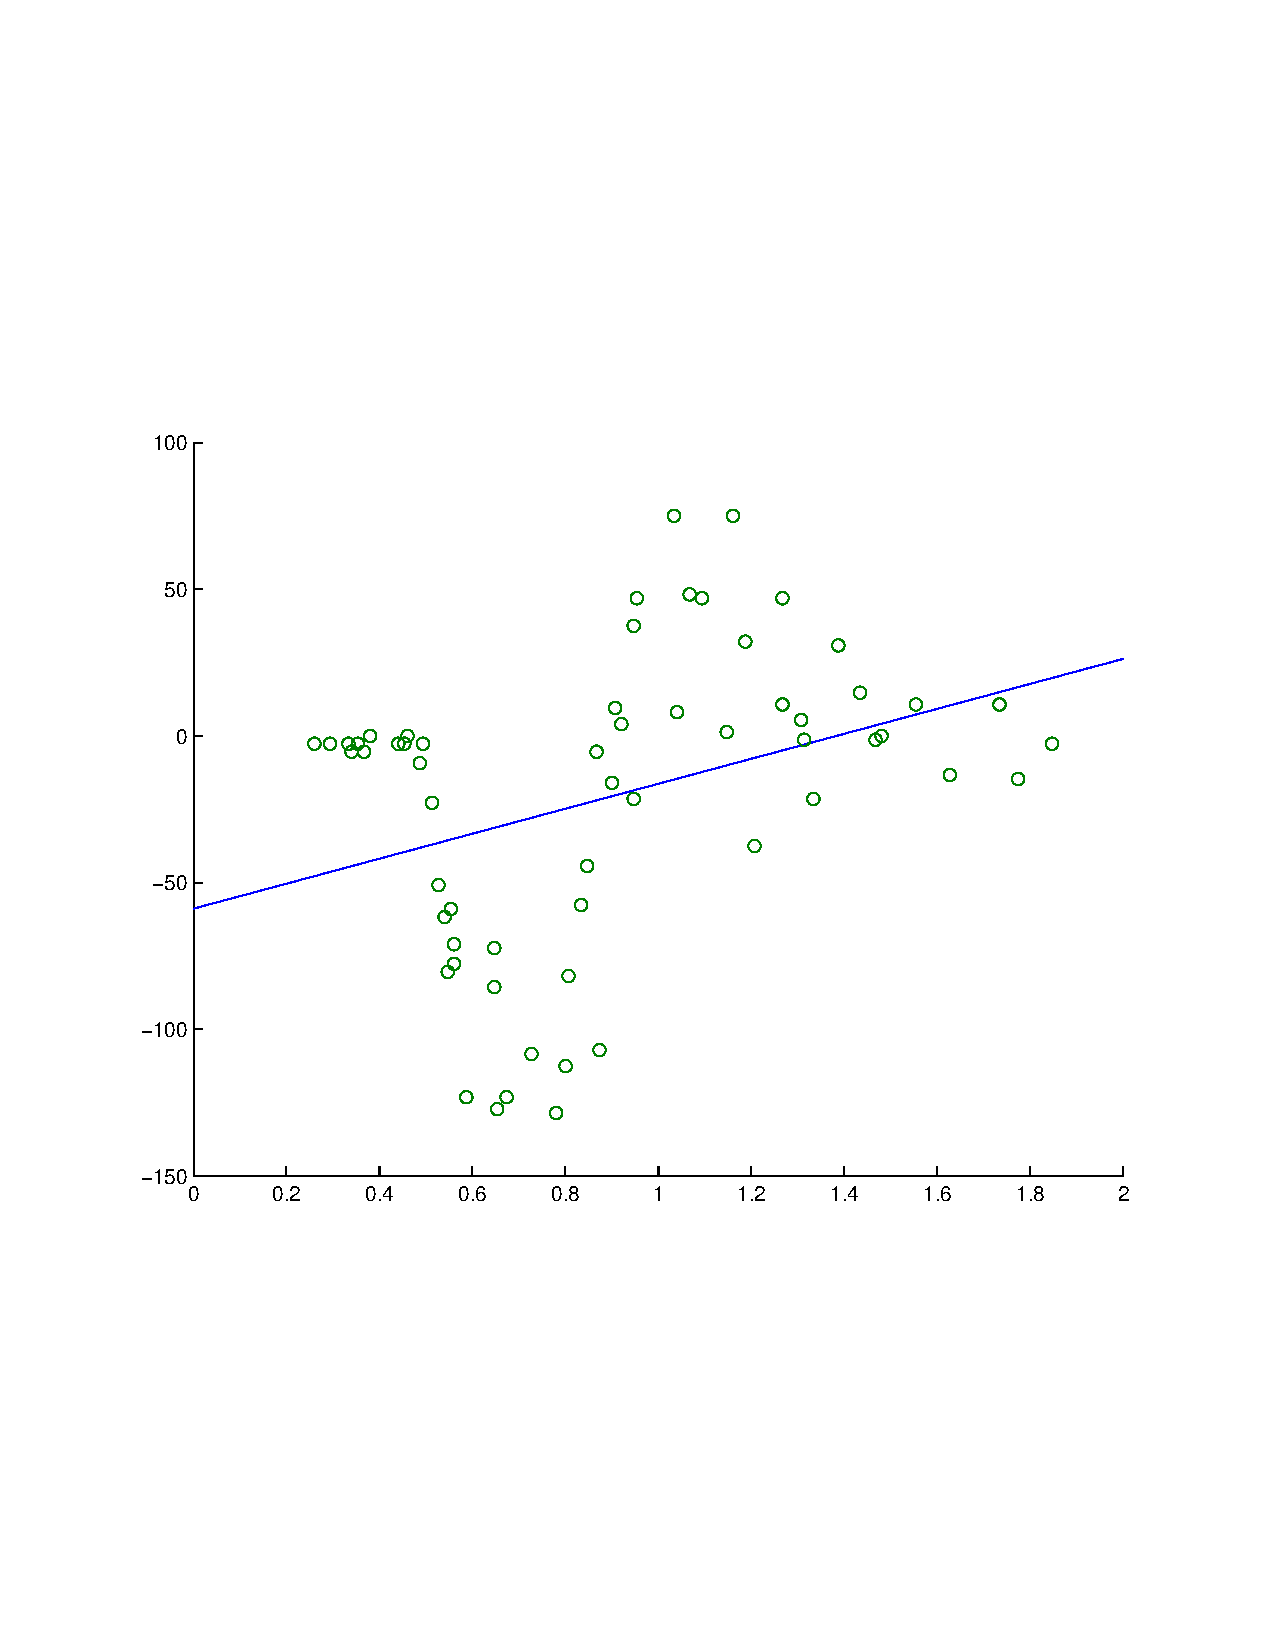
\includegraphics[width=0.5\textwidth]{\figdir/prob1b.pdf} \\
Training MSE: 2235.8 \\
Test MSE: 2414.7

\item Polynomial training errors:
\begin{figure}[h!] \centering
\begin{tabular}{cccc}
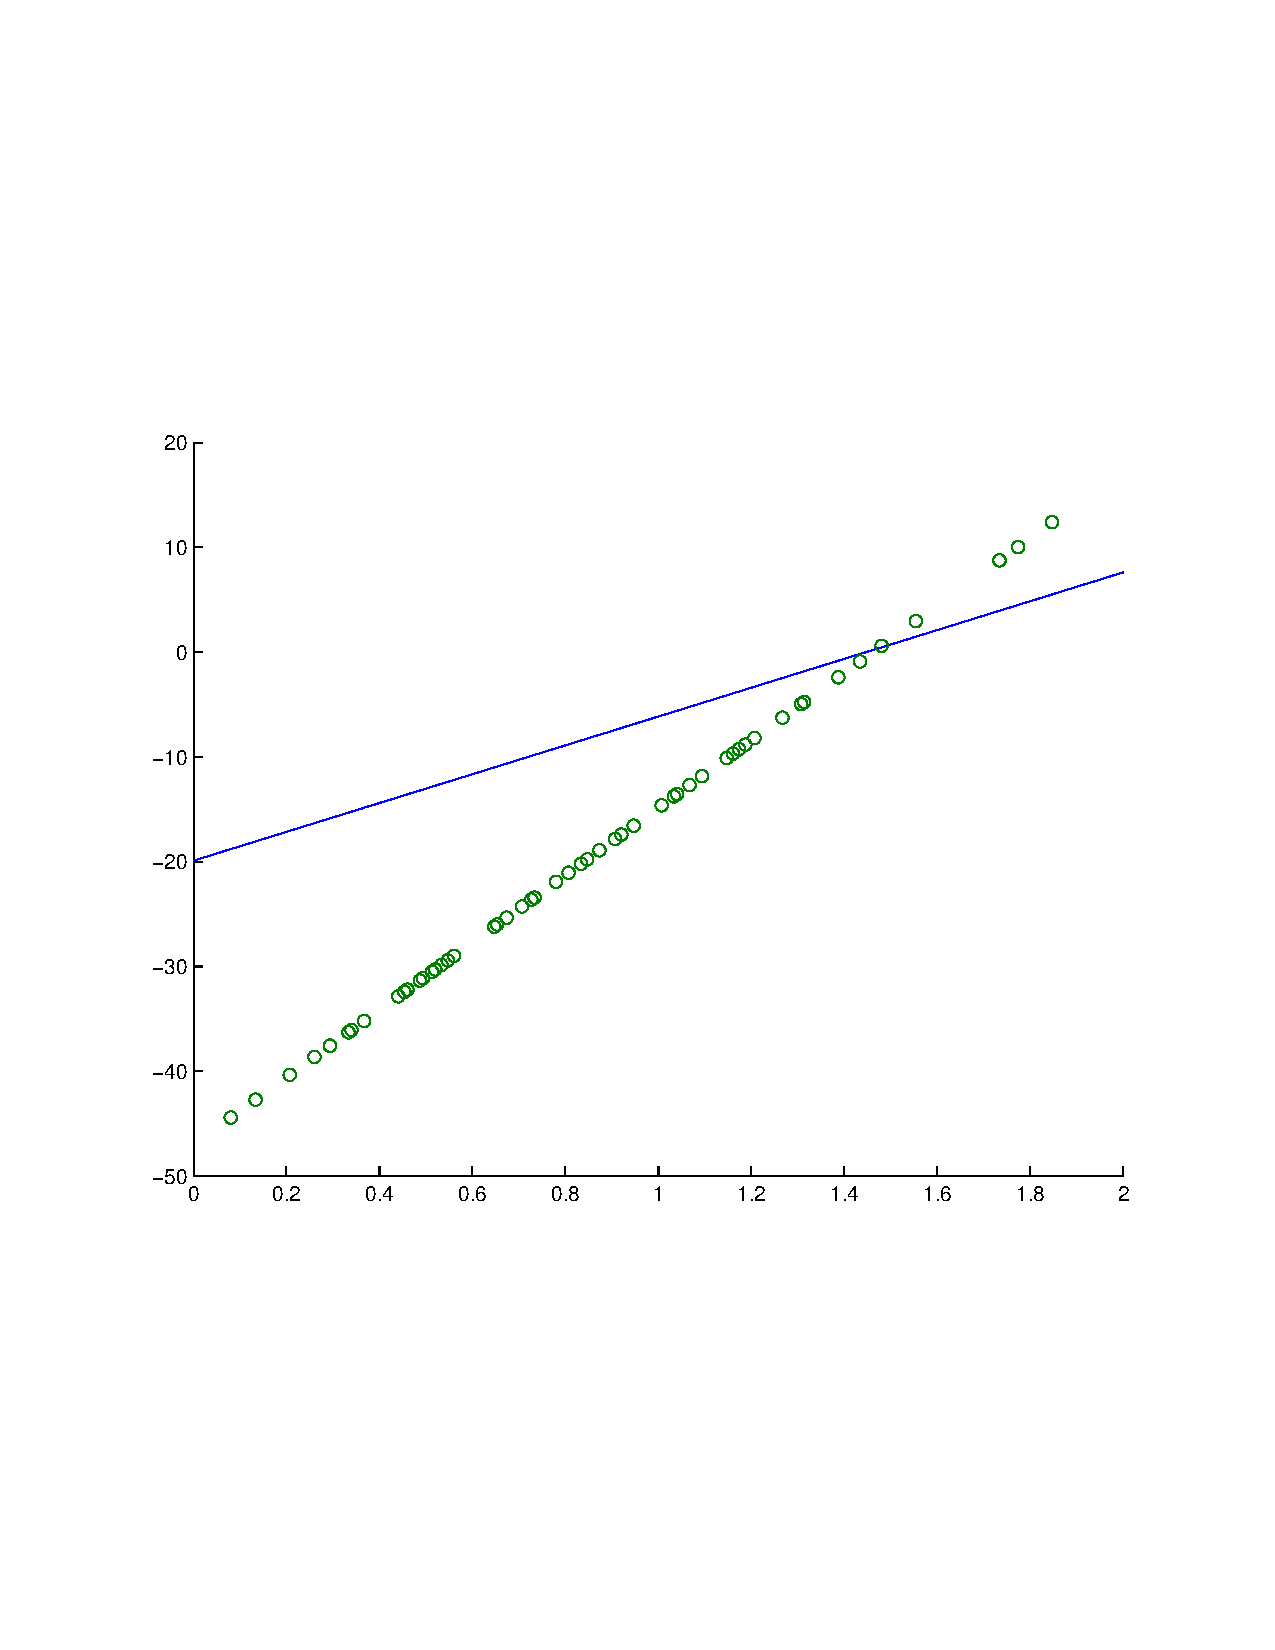
\includegraphics[width=.22\textwidth]{\figdir/prob1c_deg1} &
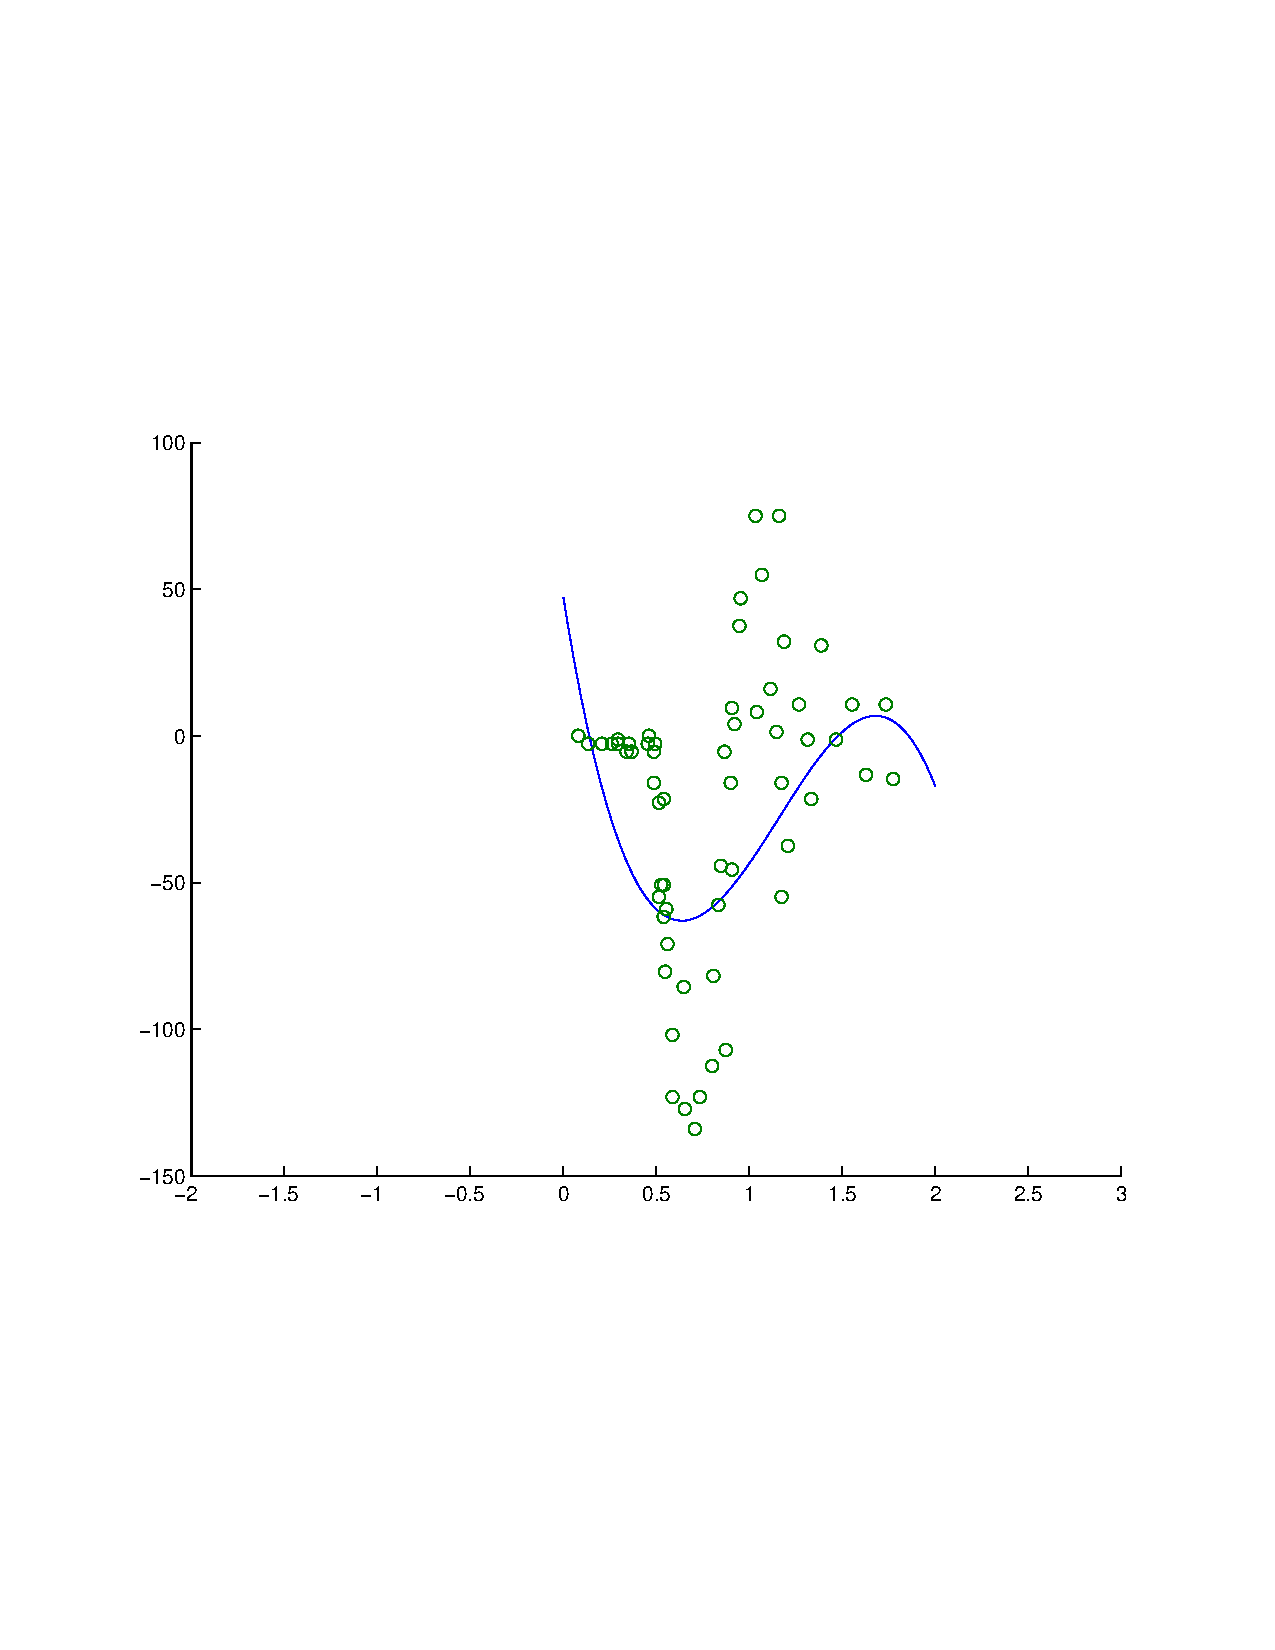
\includegraphics[width=.22\textwidth]{\figdir/prob1c_deg3} &
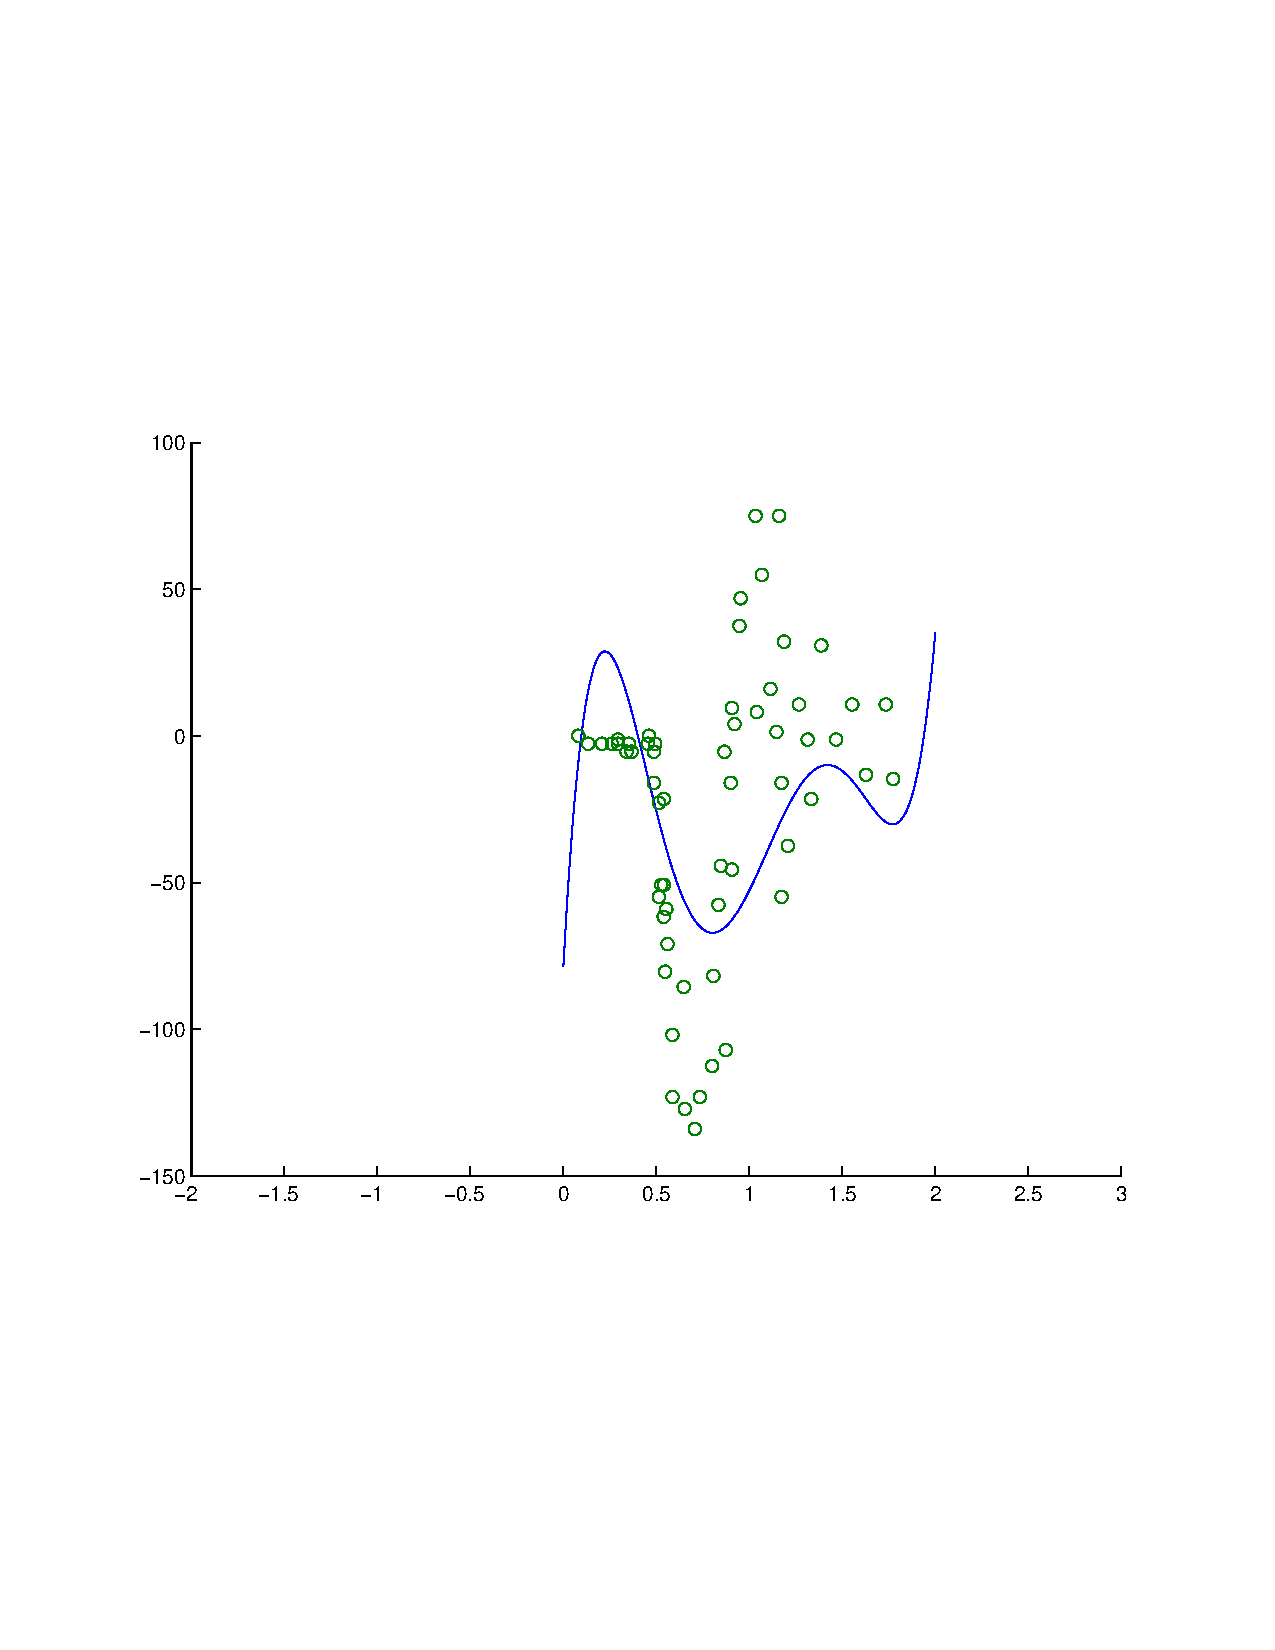
\includegraphics[width=.22\textwidth]{\figdir/prob1c_deg5} &
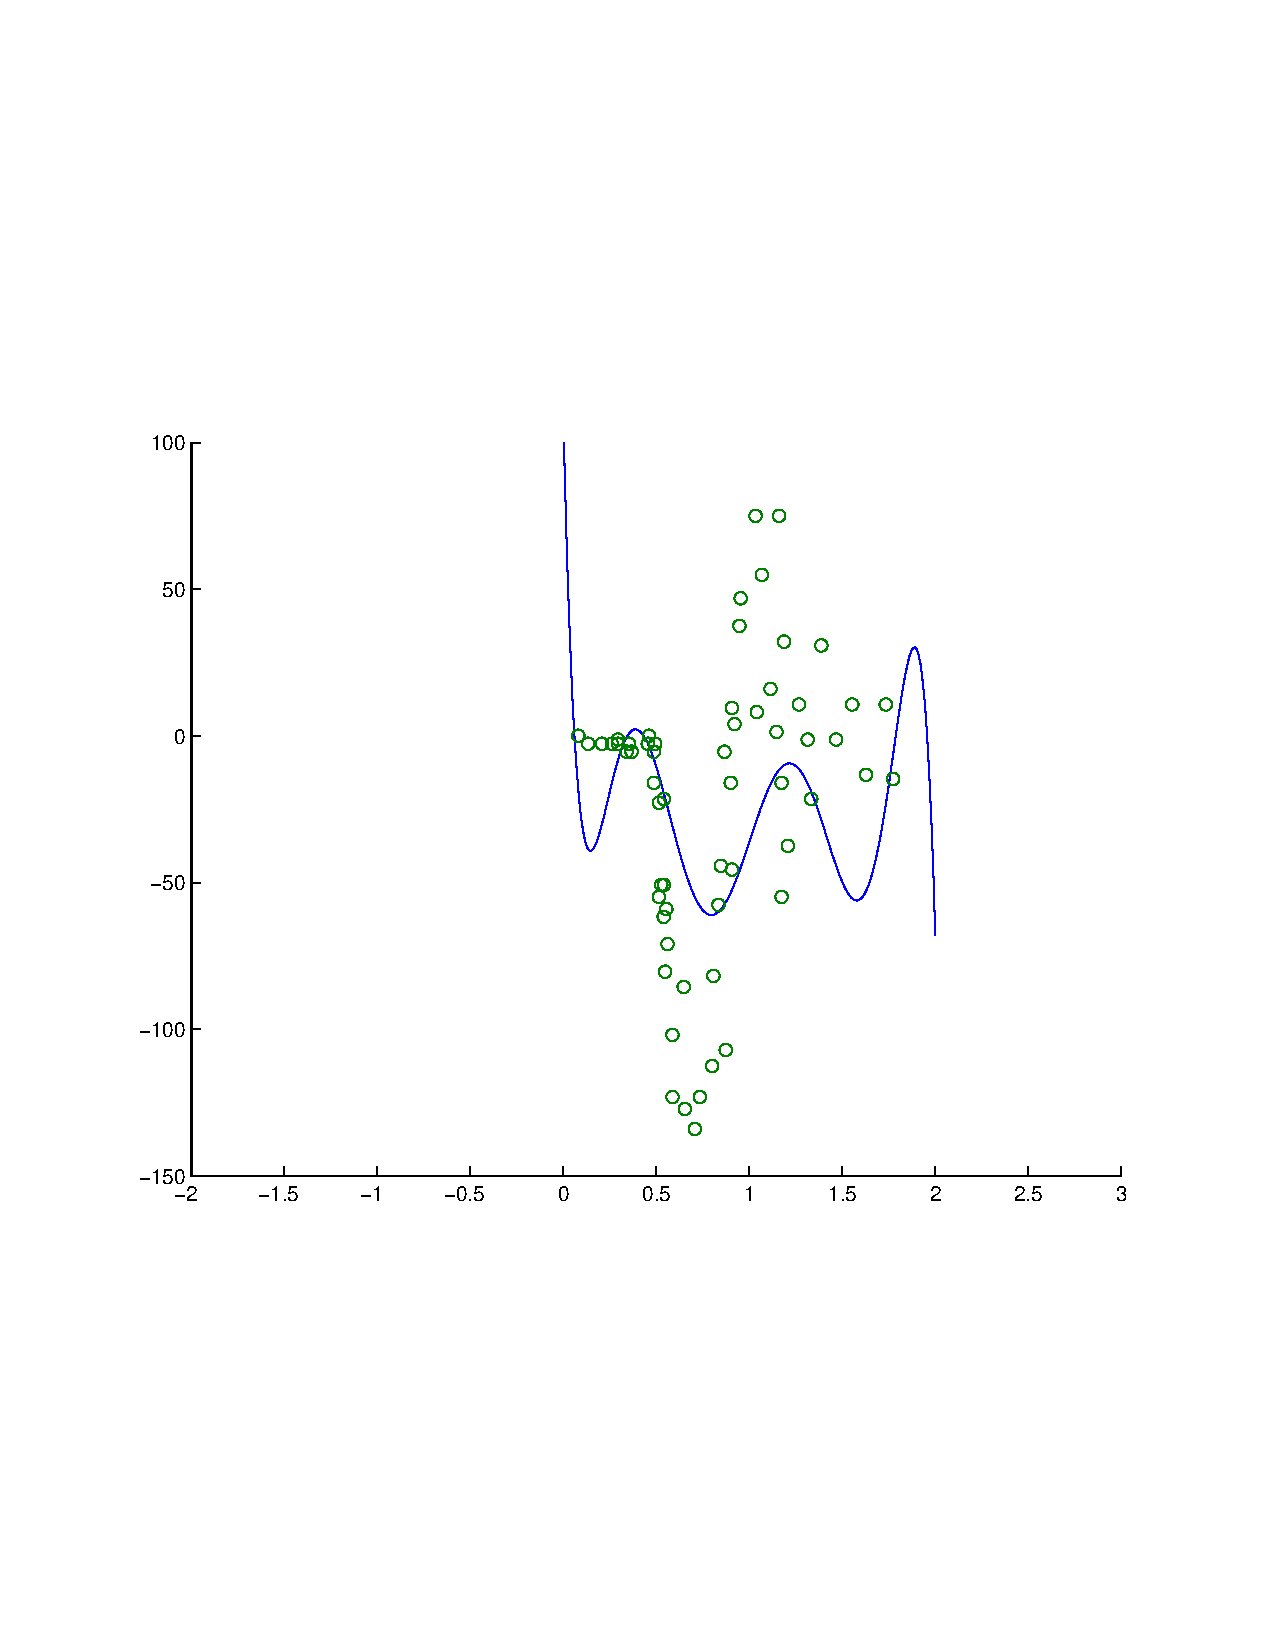
\includegraphics[width=.22\textwidth]{\figdir/prob1c_deg7} \\
1 & 3 & 5 & 7 \\
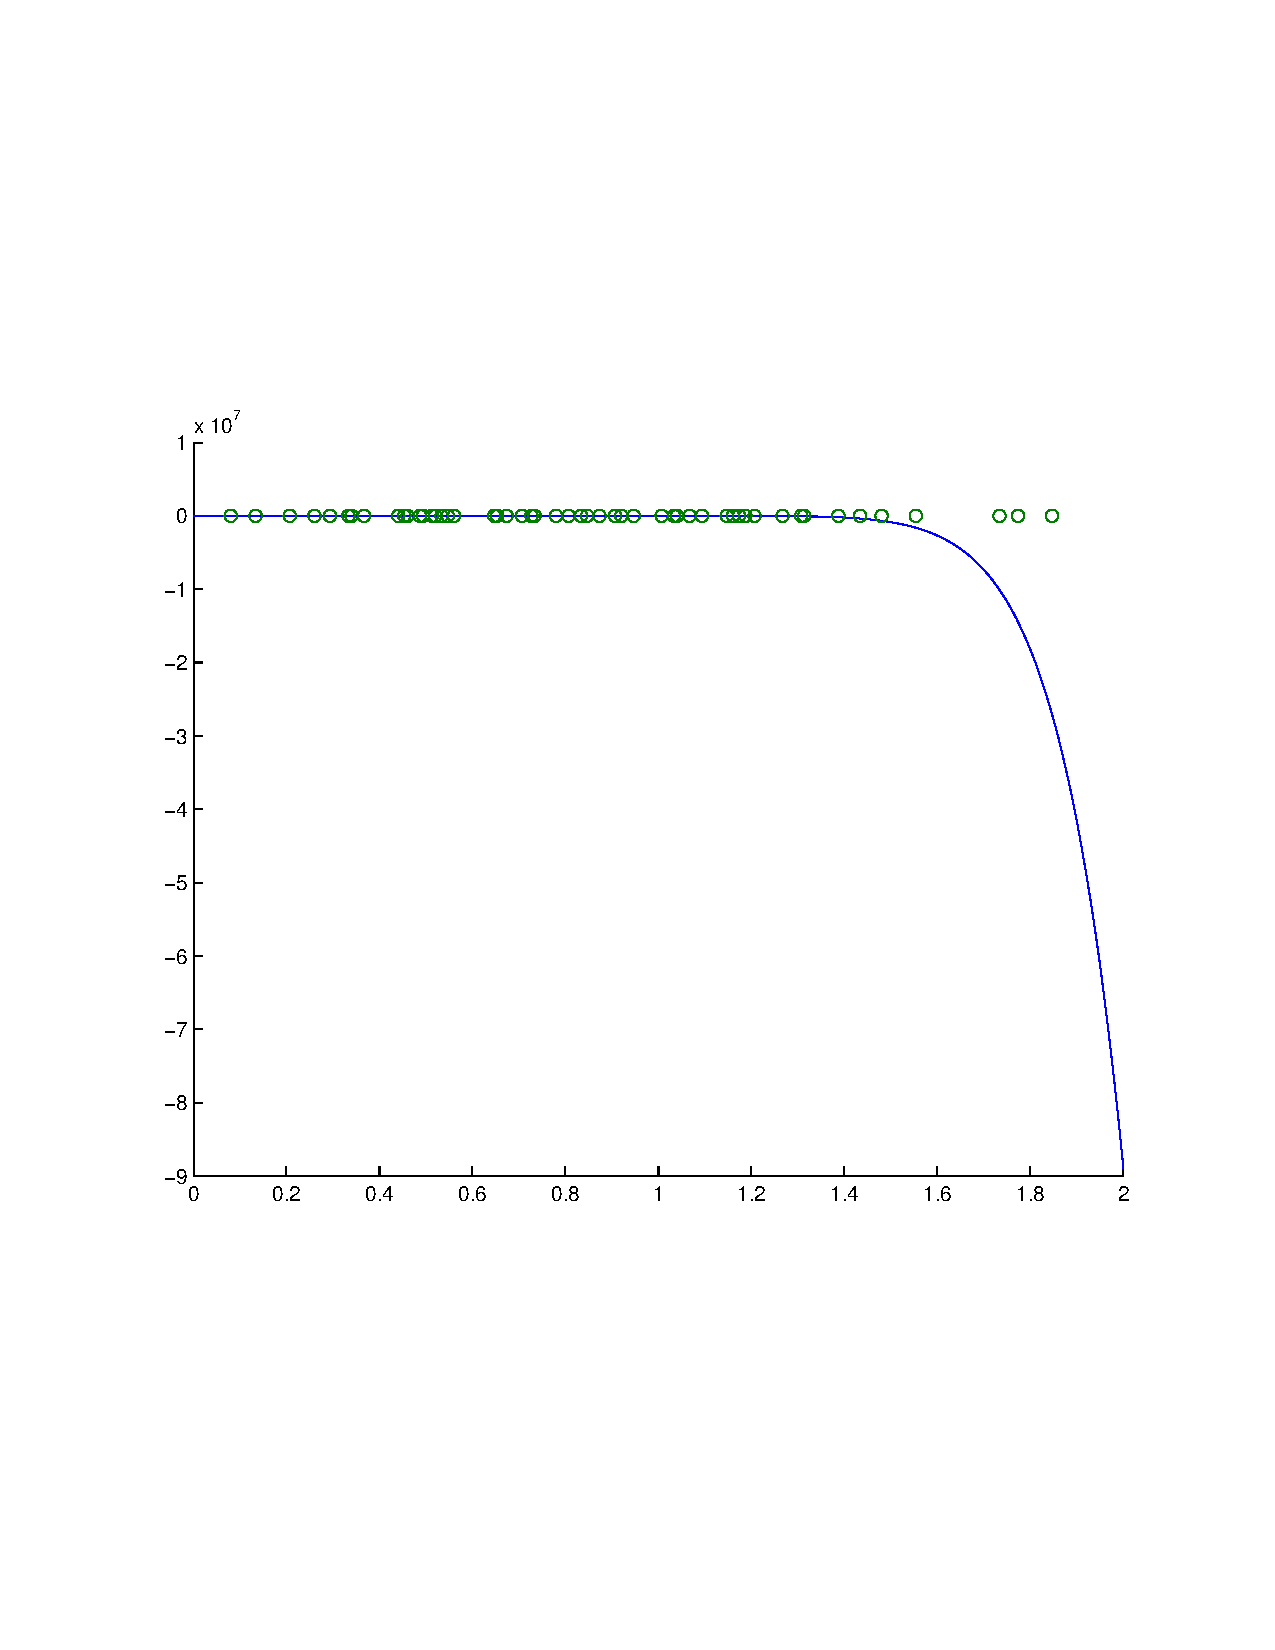
\includegraphics[width=.22\textwidth]{\figdir/prob1c_deg10} &
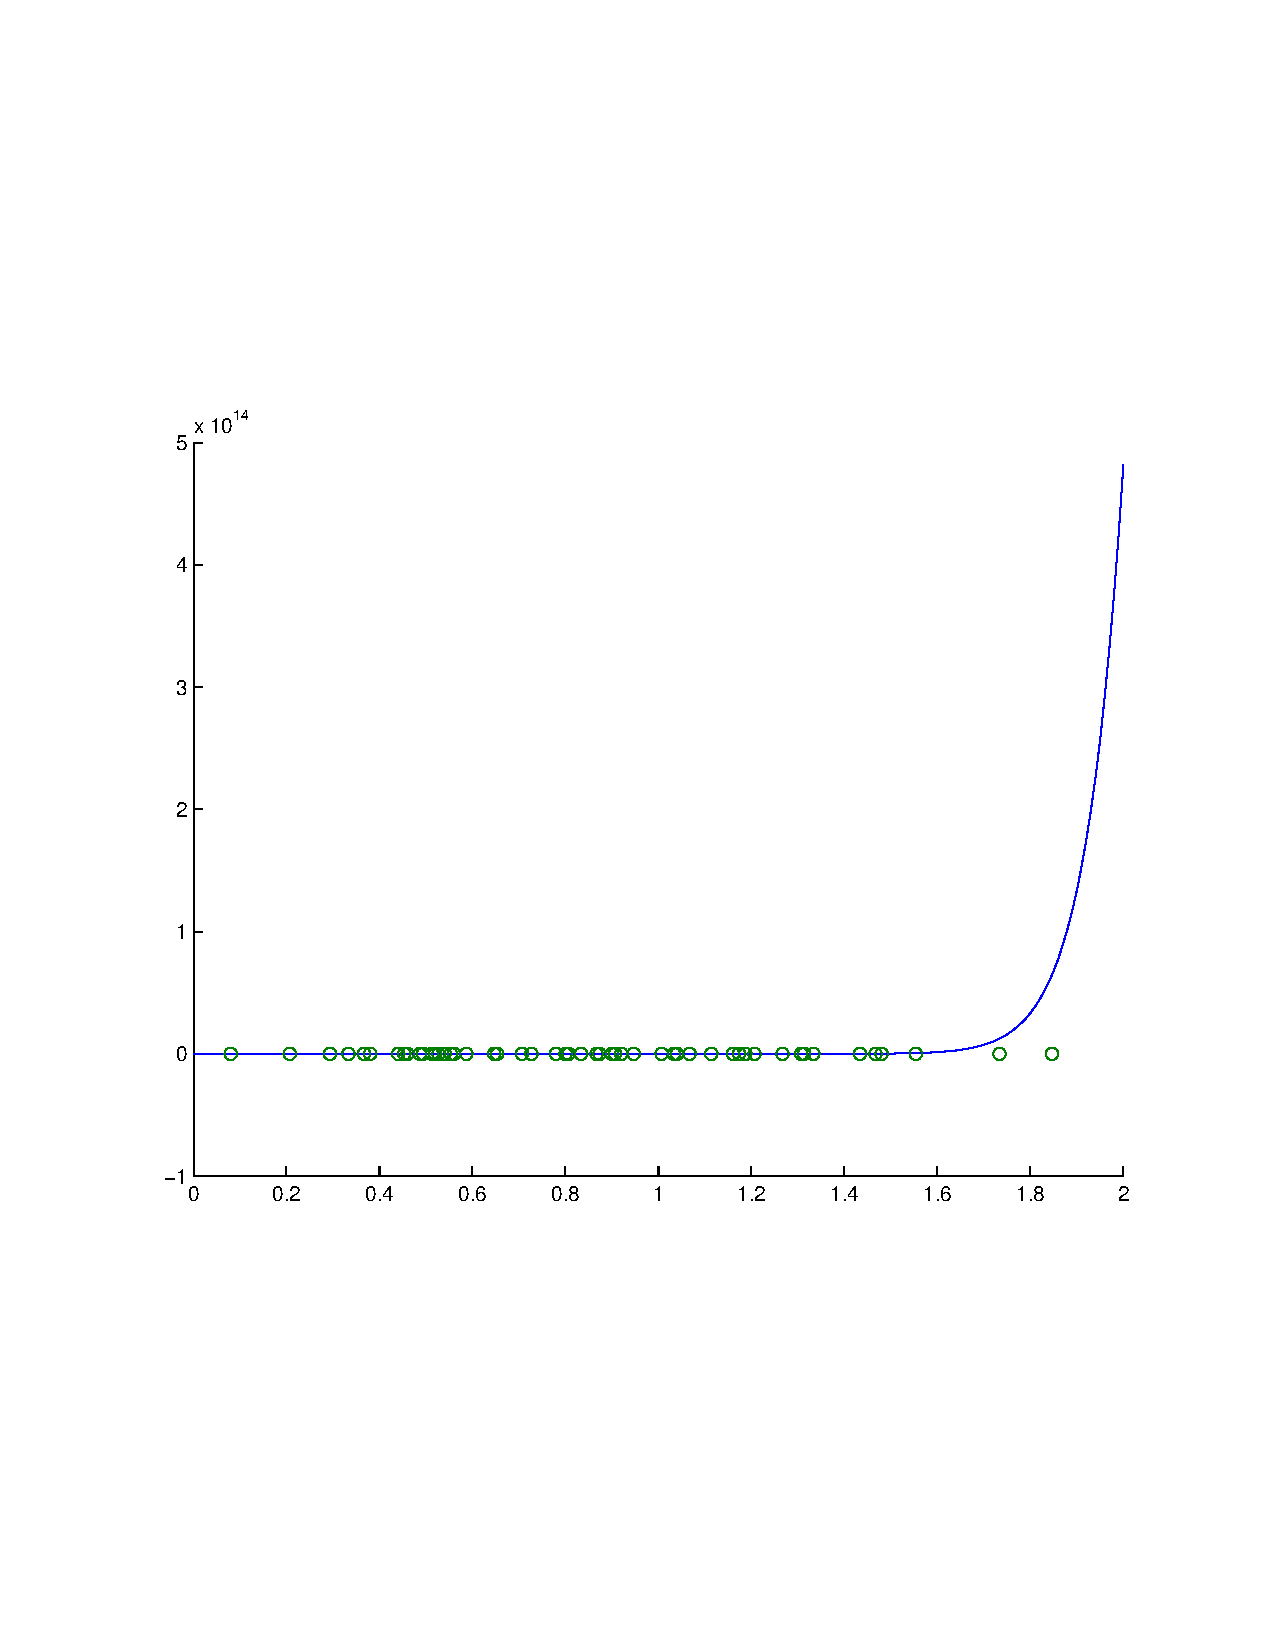
\includegraphics[width=.22\textwidth]{\figdir/prob1c_deg18} &
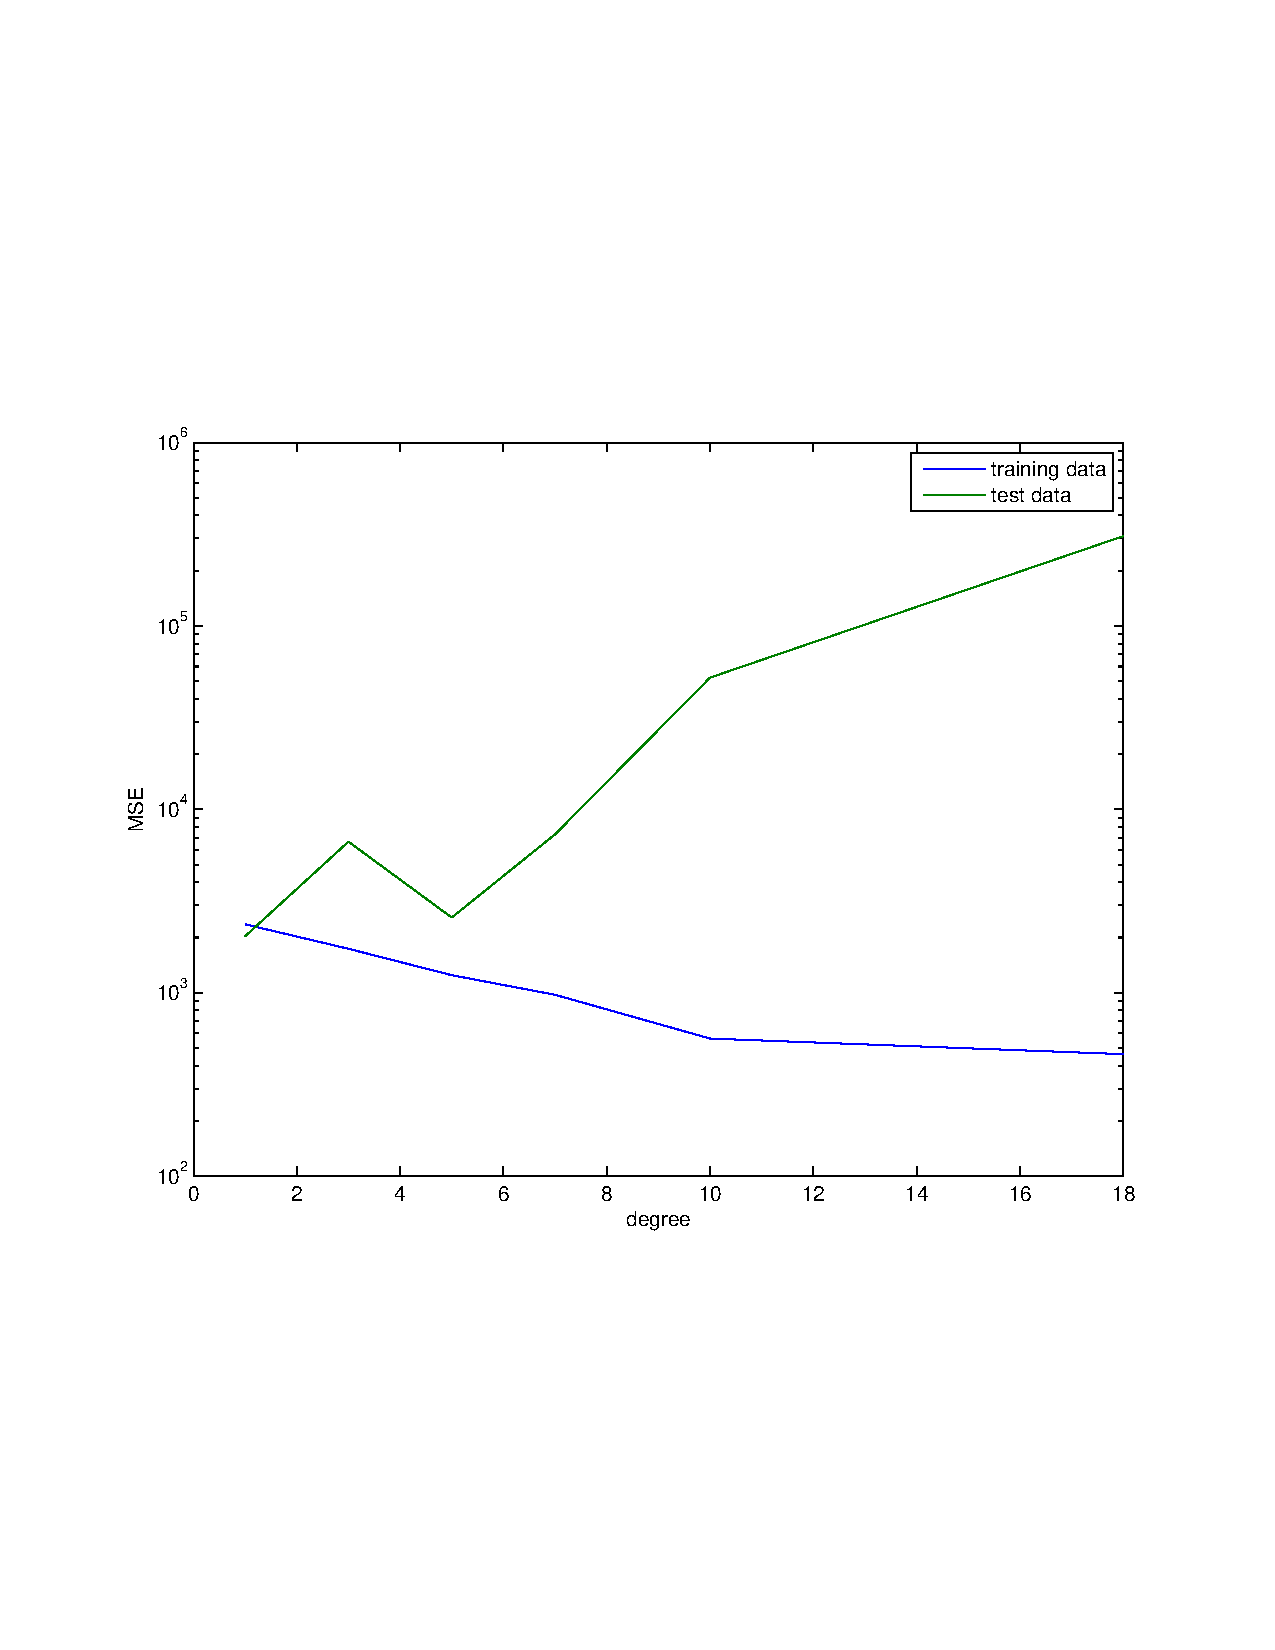
\includegraphics[width=.22\textwidth]{\figdir/prob1c_mse} \\
10 & 18 & MSE
\end{tabular}
\end{figure}

\vspace{2in} % to keep big plots from appearing on next page before this
\item 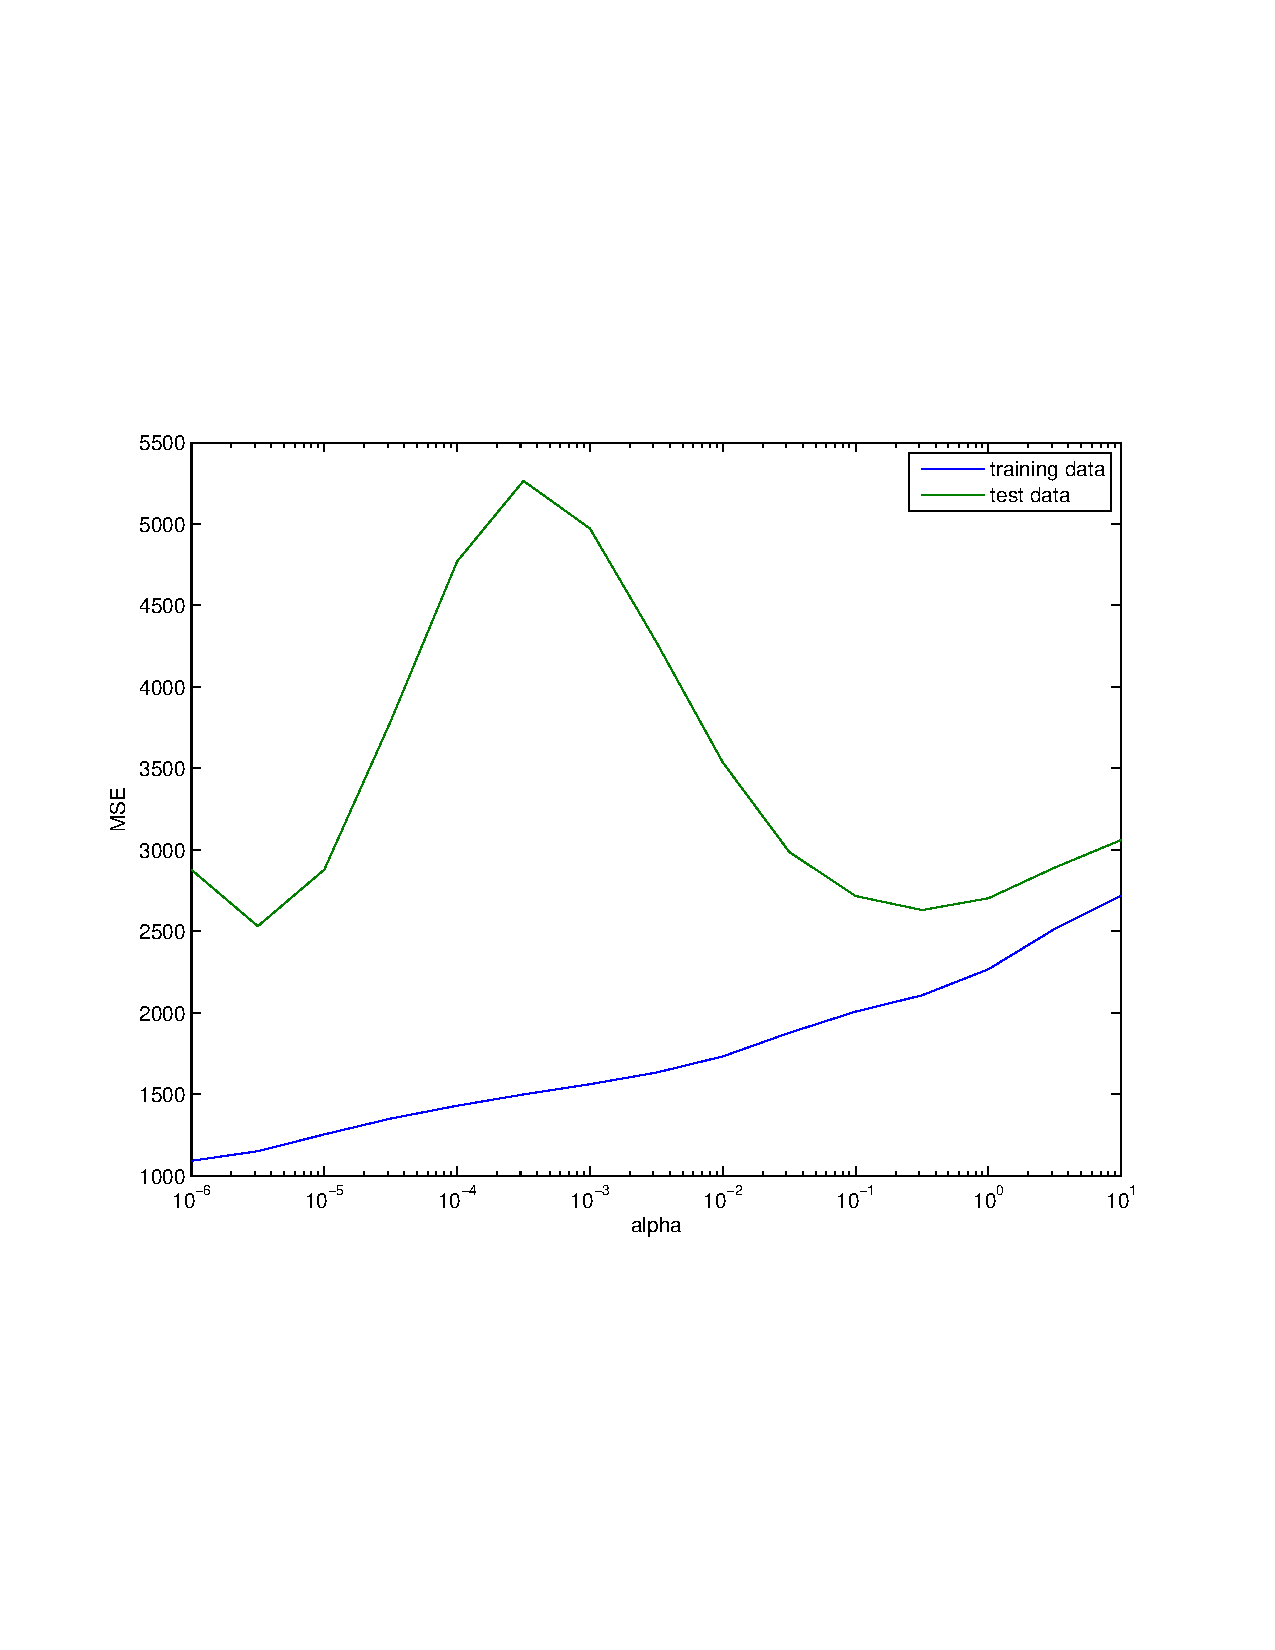
\includegraphics[width=.5\textwidth]{\figdir/prob1d}

\end{enumerate}

% % % % % % % % % % % % % % % % % % % % % % % % % % % % % % % % % % % % % % % % % % % % % % % % % % % % % % % % % % % % % % % %

\subsection*{Problem 2: Perceptron Classifiers}

\begin{enumerate}[(a)]

\item classes 0 vs. 1 (linearly separable as shown in plot) \\
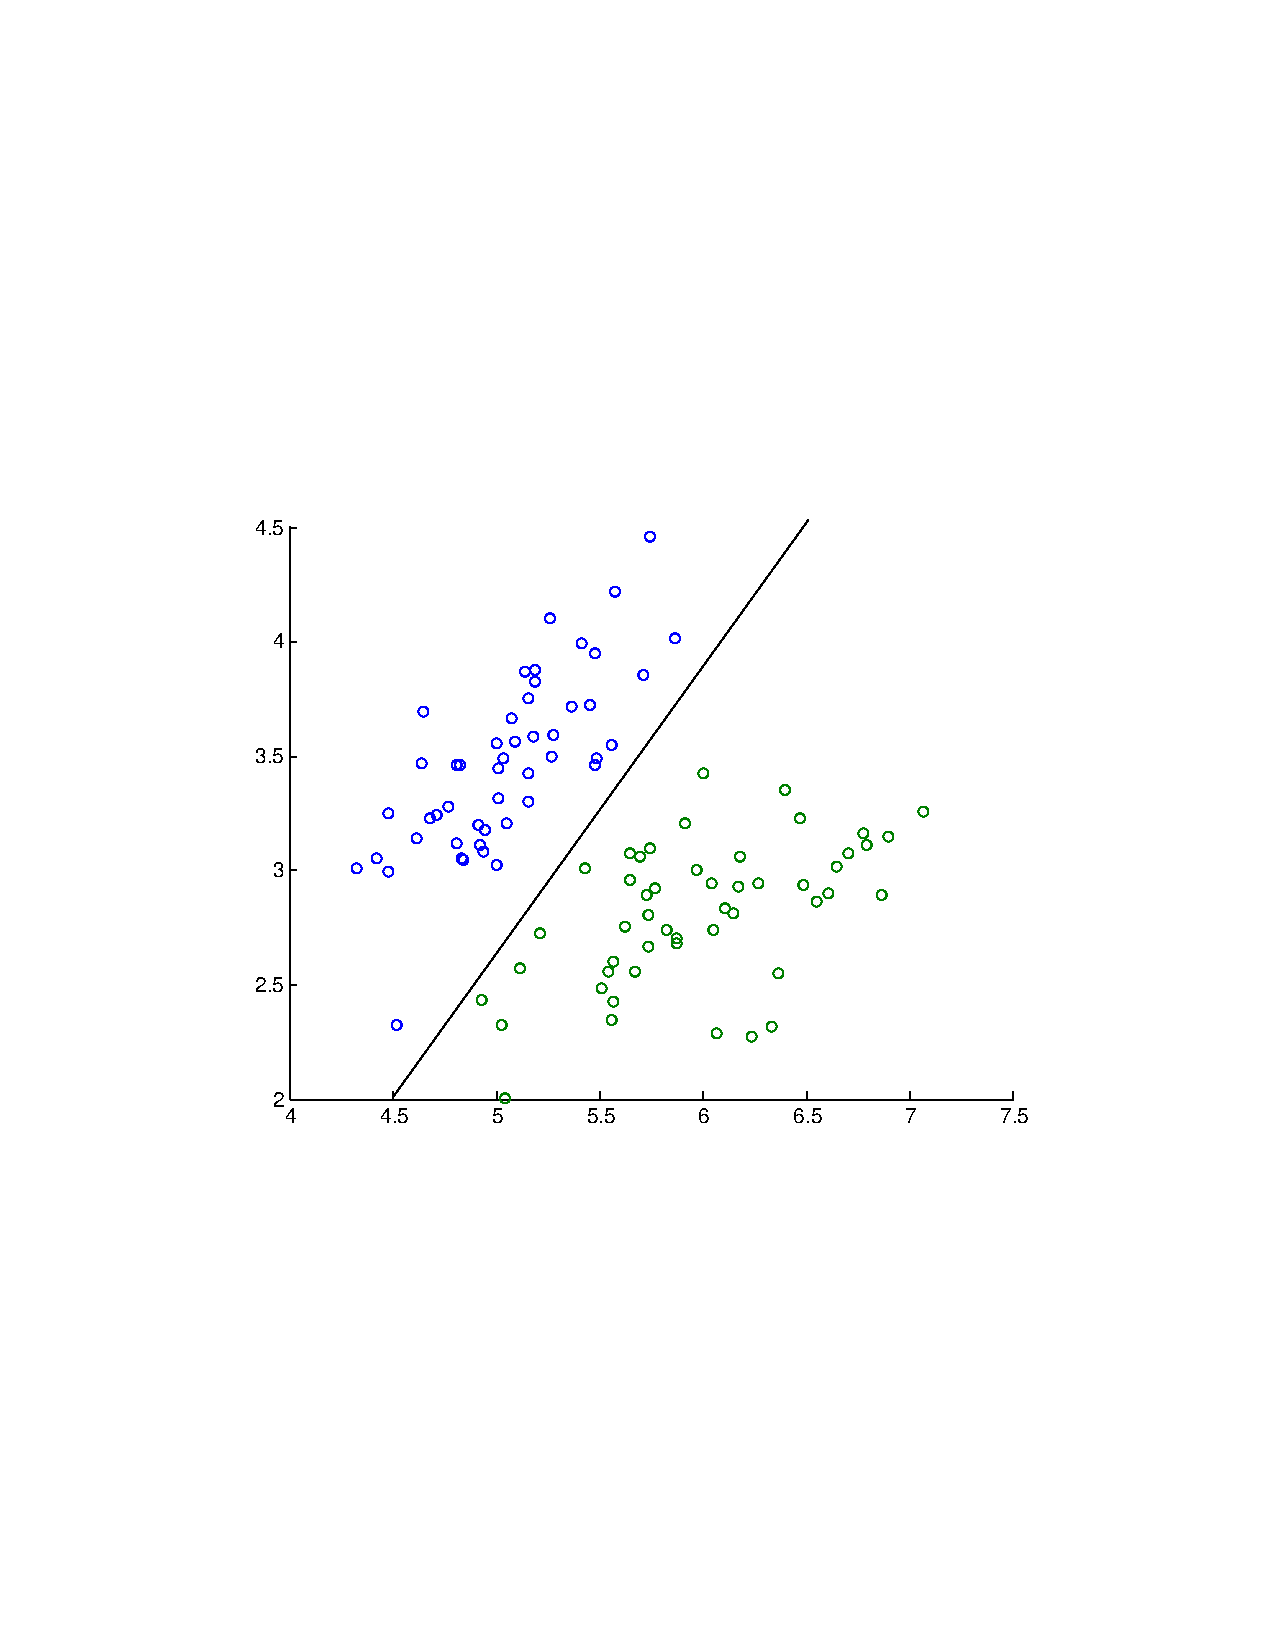
\includegraphics[width=.5\textwidth]{\figdir/prob2a_0v1} \\
classes 1 vs. 2 (not linearly separable) \\
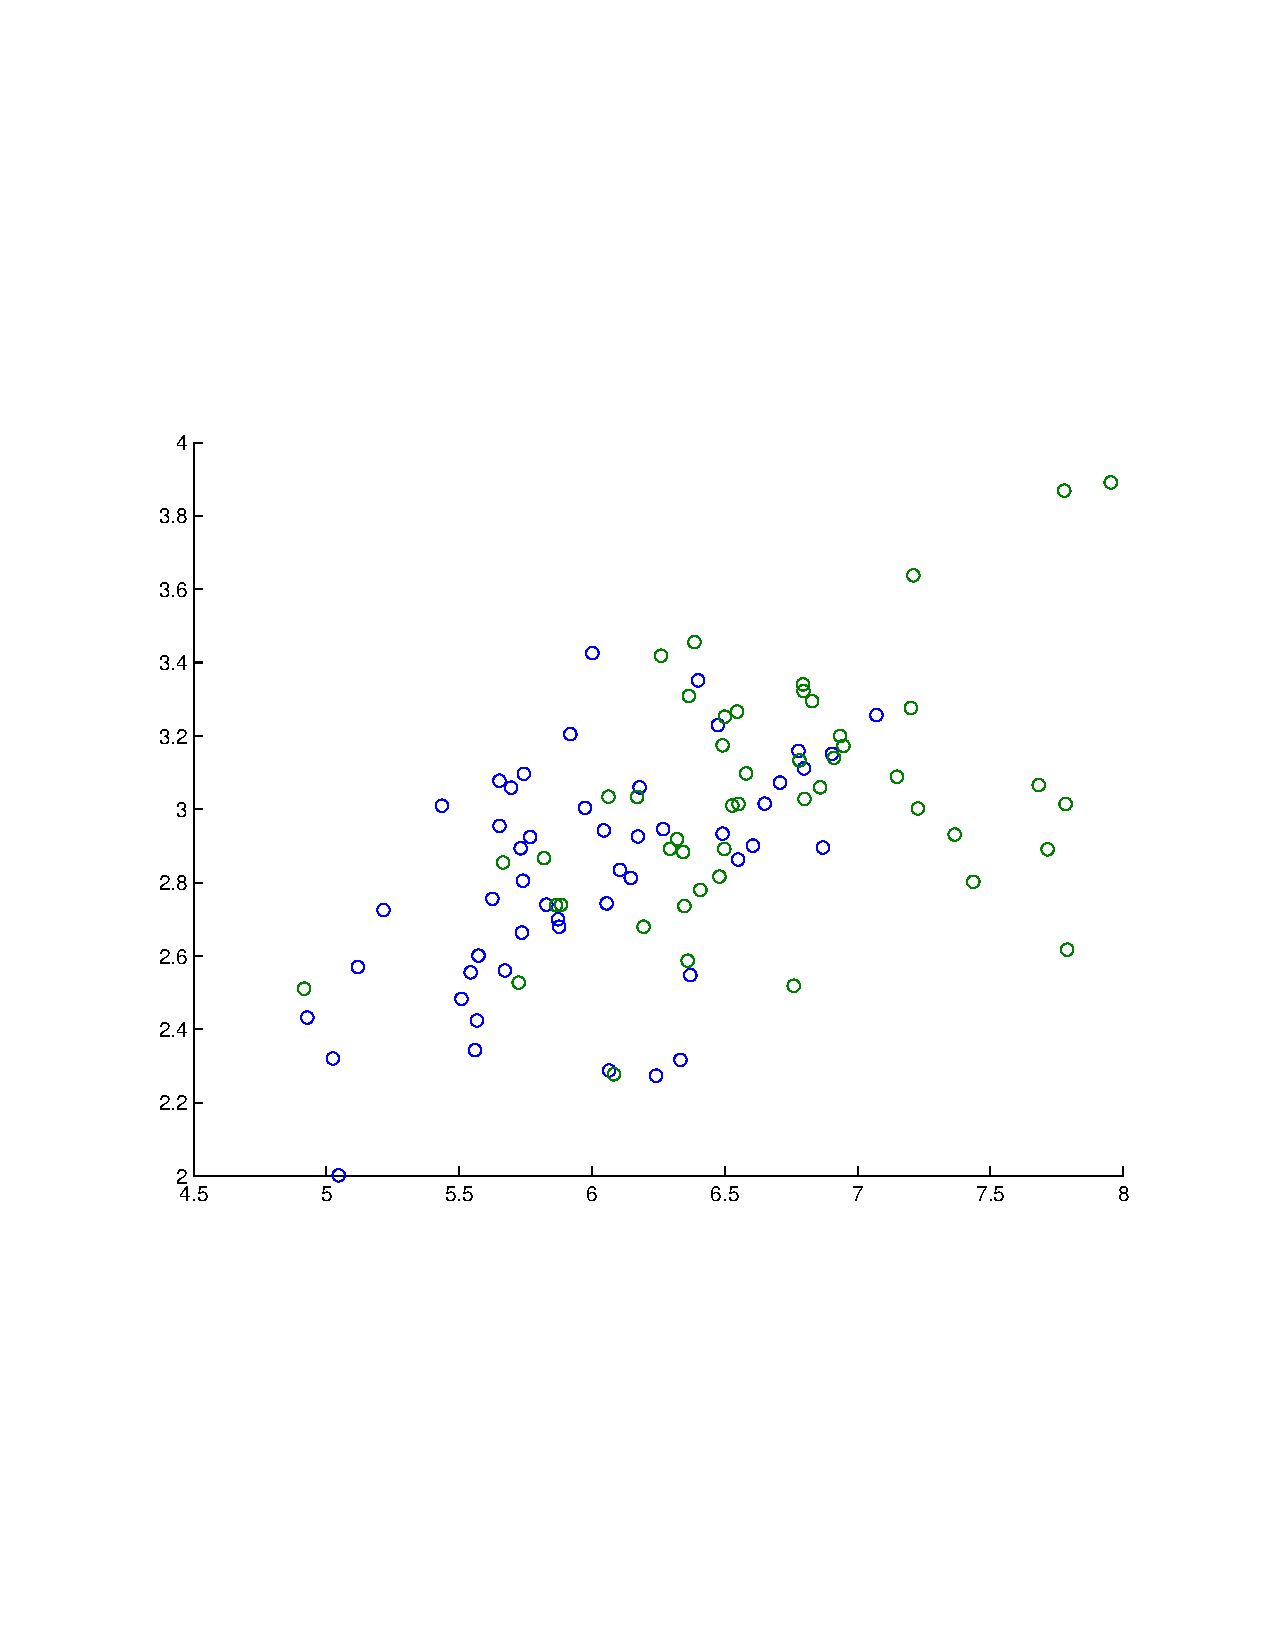
\includegraphics[width=.5\textwidth]{\figdir/prob2a_1v2} \\

\item \lstinputlisting{src/prob2.m}

\item The \textbf{XA,YA} data converged much faster than the \textbf{XB,YB} data.
The former also reached a pretty good error rate, due to it being linearly separable, as opposed to the latter that never got much better than 0.5, which is the same as a random guess.
\begin{figure}[h!] \centering
\begin{tabular}{cccc}
0 vs. 1 & 1 vs. 2 \\
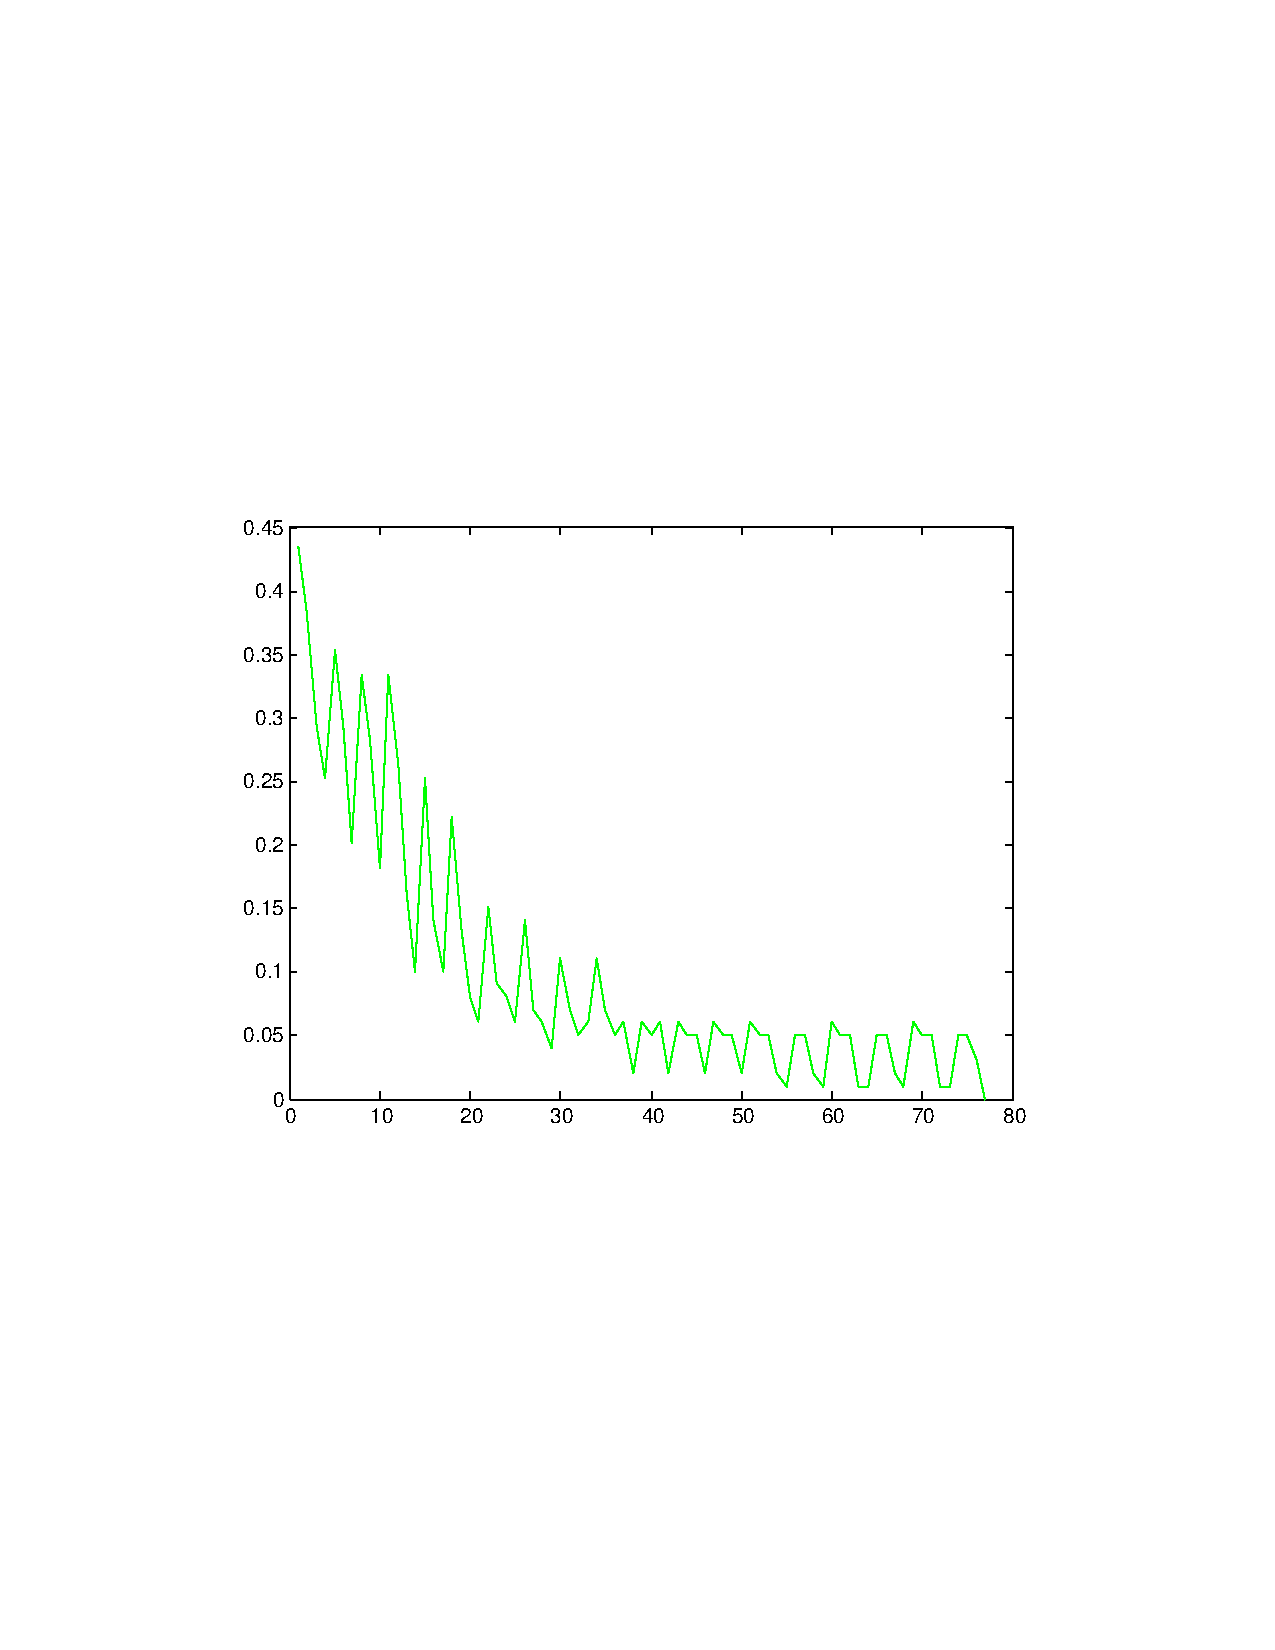
\includegraphics[width=.5\textwidth]{\figdir/prob2c_0v1.pdf} &
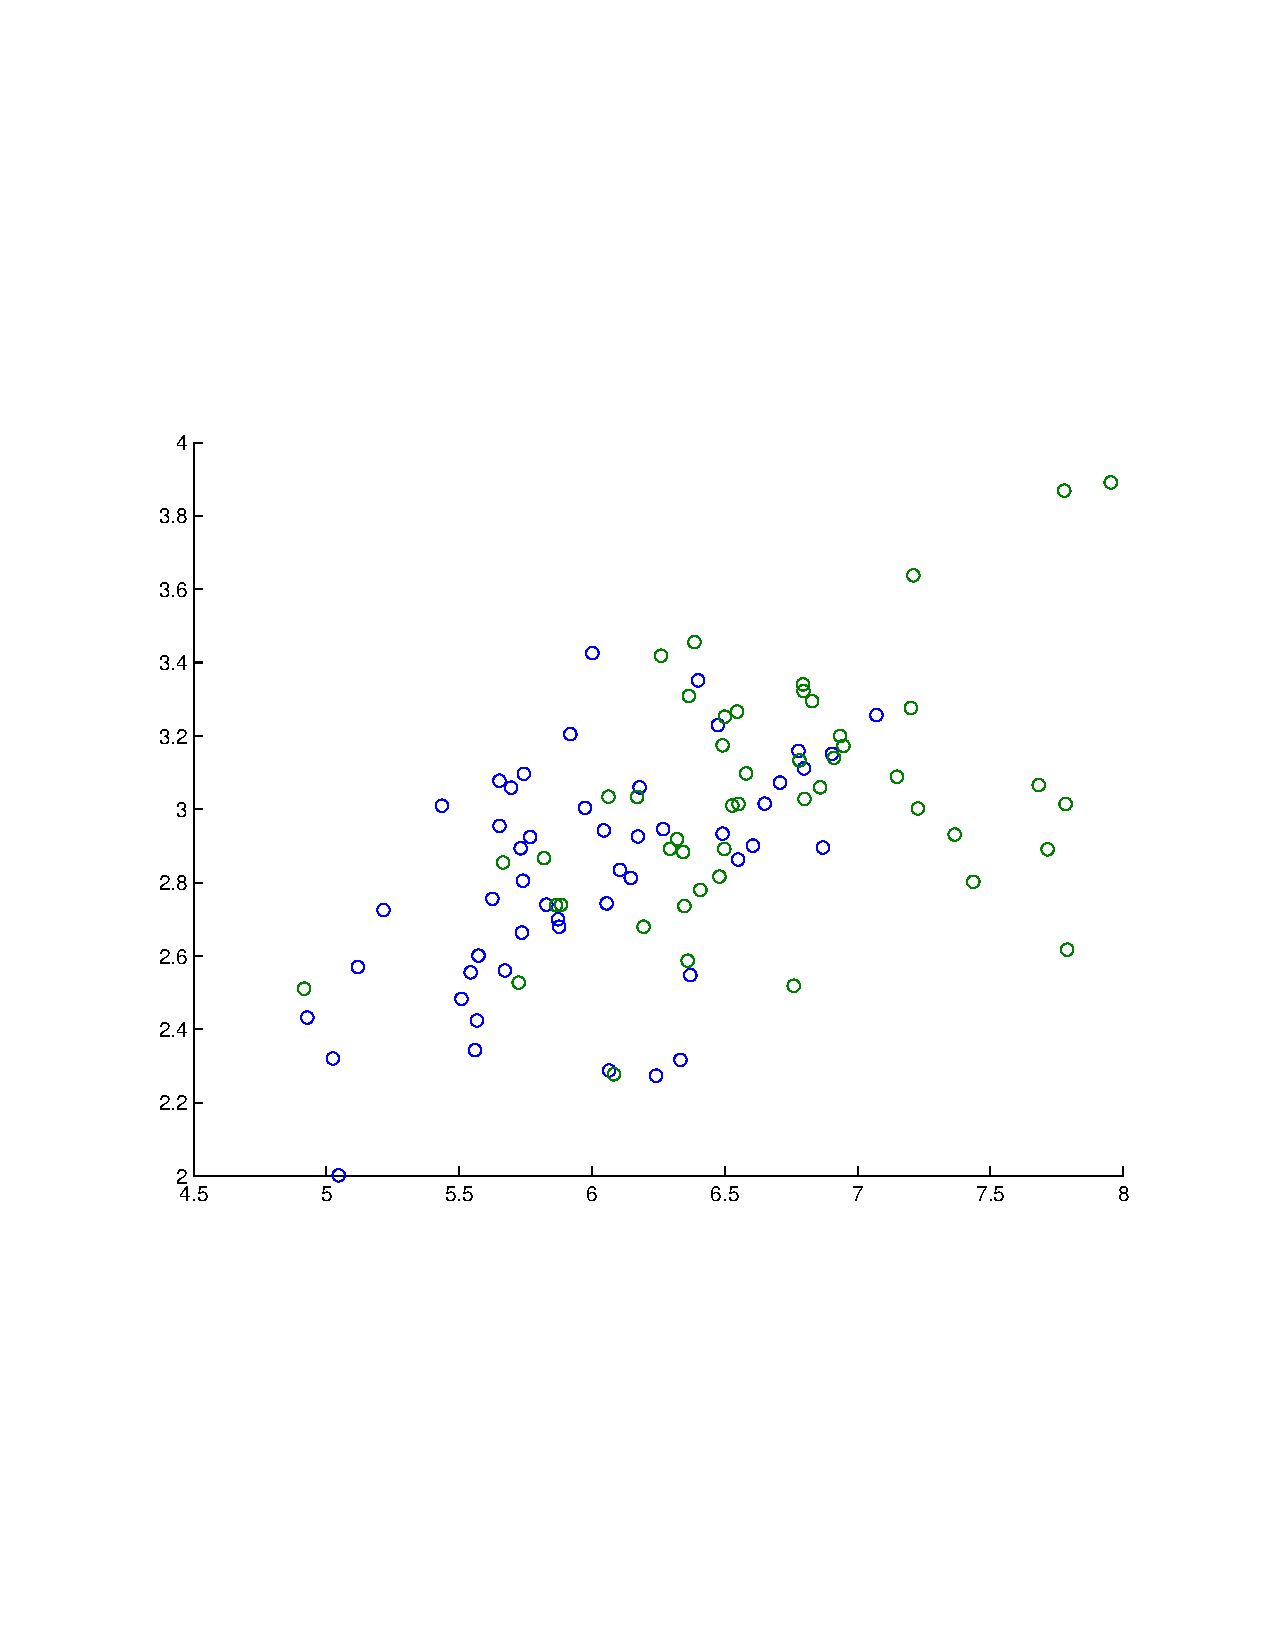
\includegraphics[width=.5\textwidth]{\figdir/prob2c_1v2.pdf}
\end{tabular}
\end{figure}

\begin{figure}[h!] \centering
\begin{tabular}{cccc}
0 vs. 1 & 1 vs. 2 \\
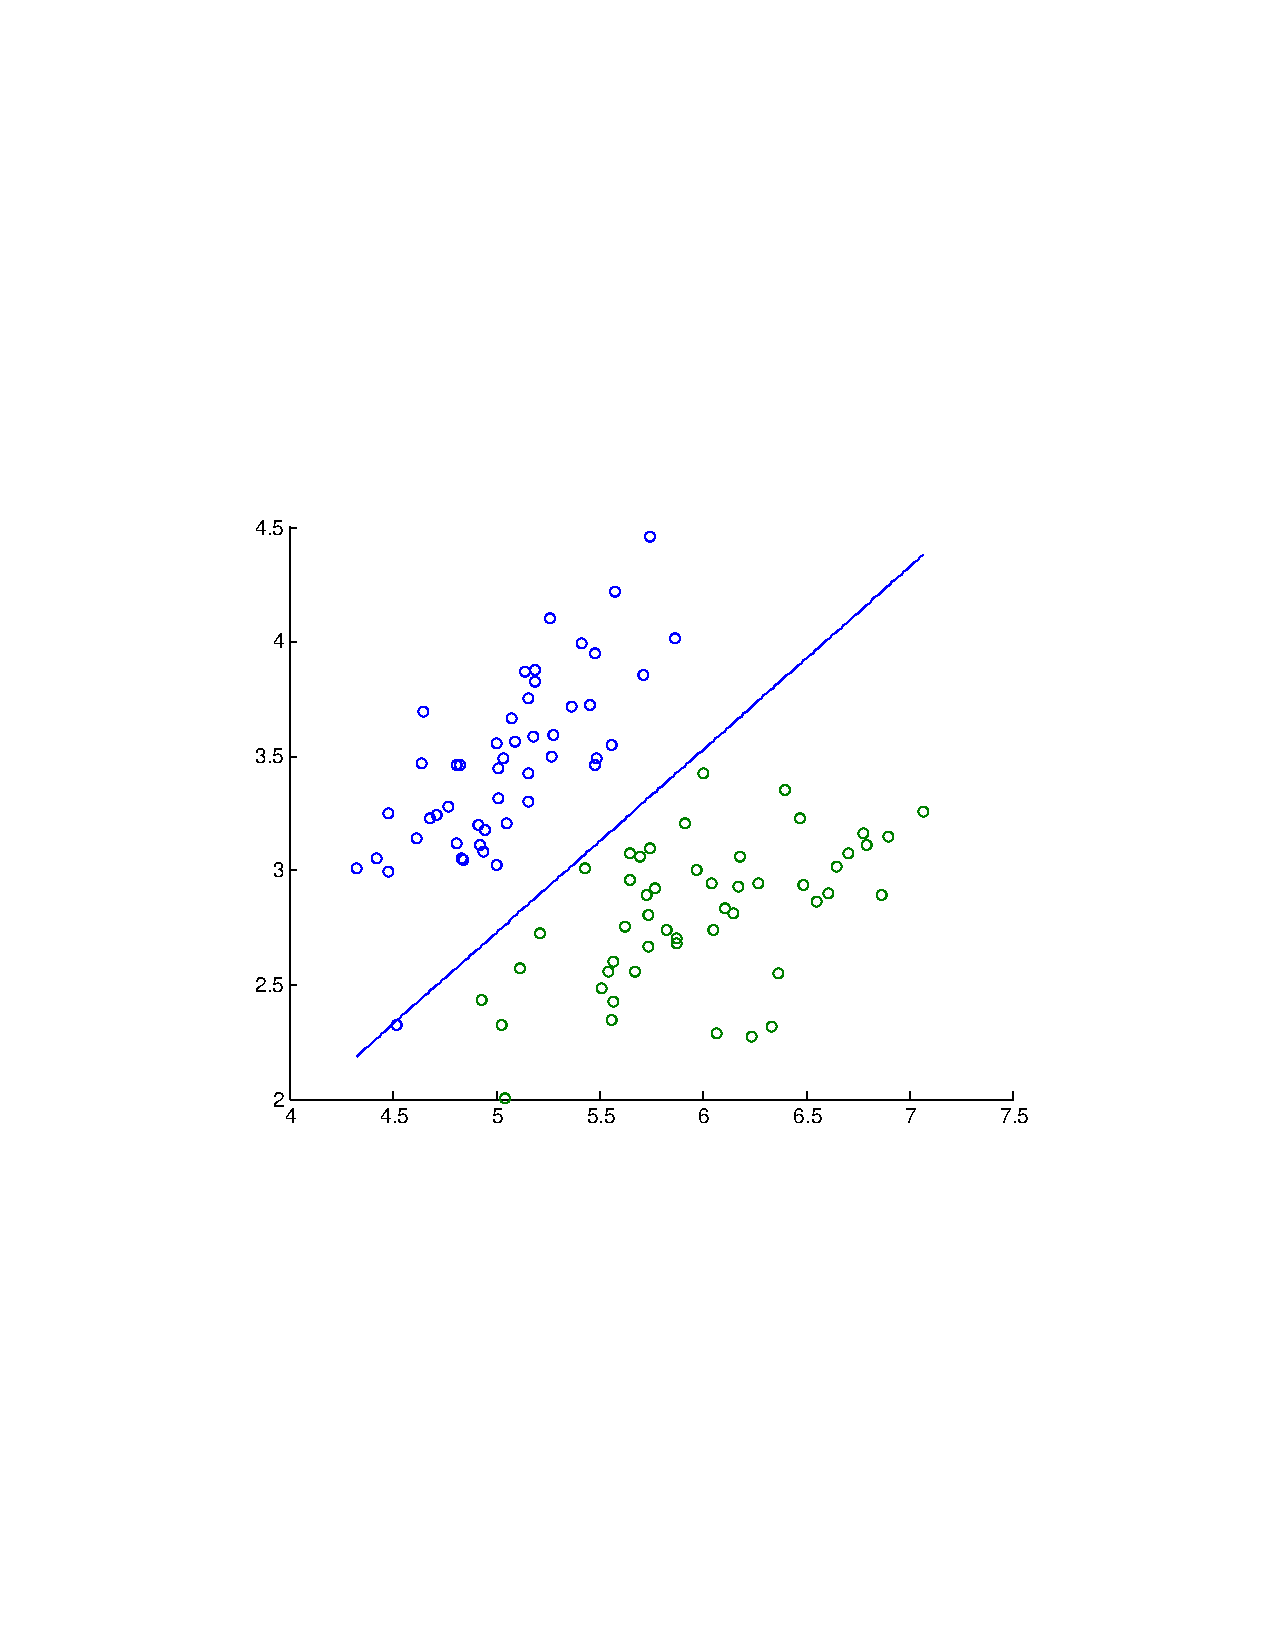
\includegraphics[width=.5\textwidth]{\figdir/prob2d_0v1.pdf} &
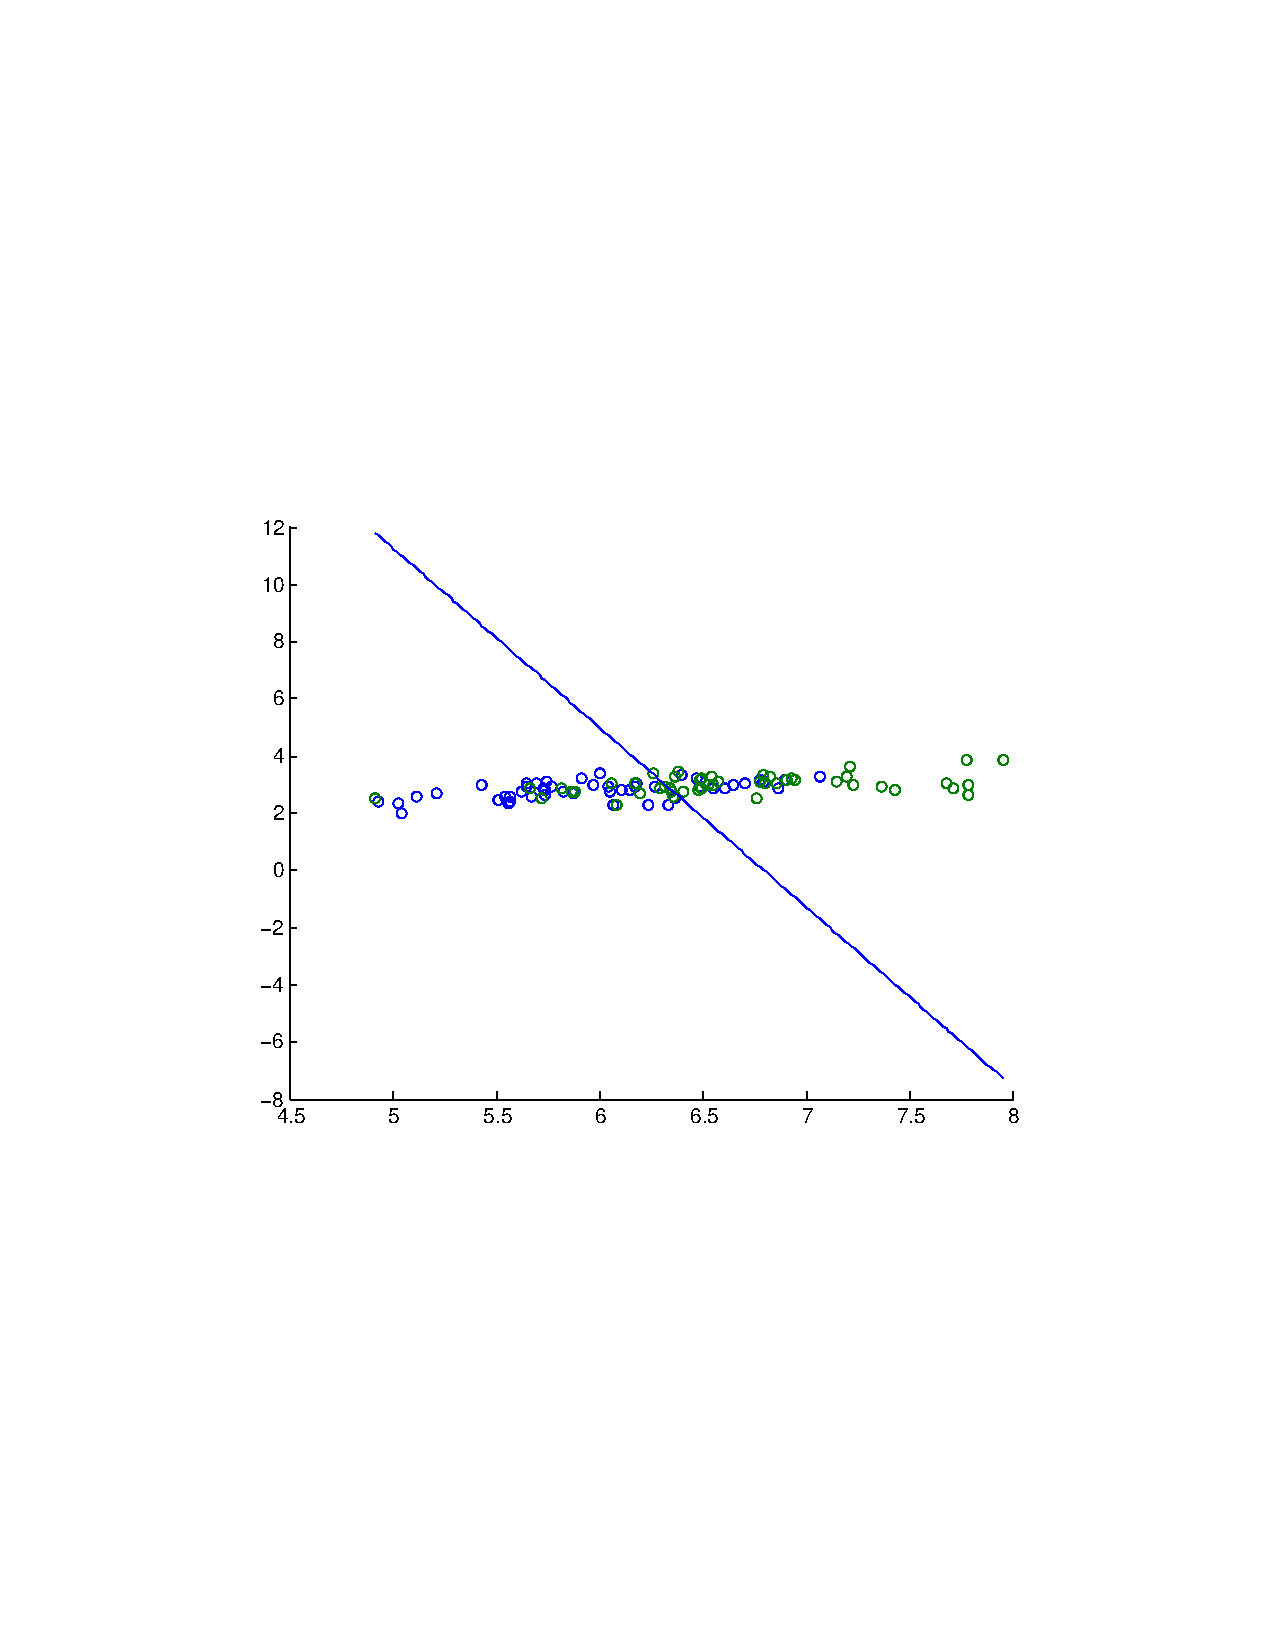
\includegraphics[width=.5\textwidth]{\figdir/prob2d_1v2.pdf}
\end{tabular}
\end{figure}

\item The \textbf{XA,YA} data actually resulted in a higher error rate (0.0101) when using weights from a linear regression.
This perceptron algorithm is able to take a step so that the decision boundary gets the blue point in the bottom left of the plots correctly, whereas the linear regression will simply try to find a rough center of mass between the data, which might miss some of the points near the ideal boundary.

The \textbf{XB,YB} data seemed to actually perform better than the perceptron algorithm with an error rate of 0.2626.
This is likely due to the linear regression finding a reasonable center, whereas the perceptron algorithm frequently gets stuck in very unsuitable situations due to the mingling of the data with respect to their classes.

\item The error actually increased in the linear regression case (1st image below) due to the new point being so far away from the rest and skewing the center that the regression algorithm was looking for.
It didn't affect the perceptron algorithm because it was in the correct direction as the rest of the points, and so was quickly classified correctly.

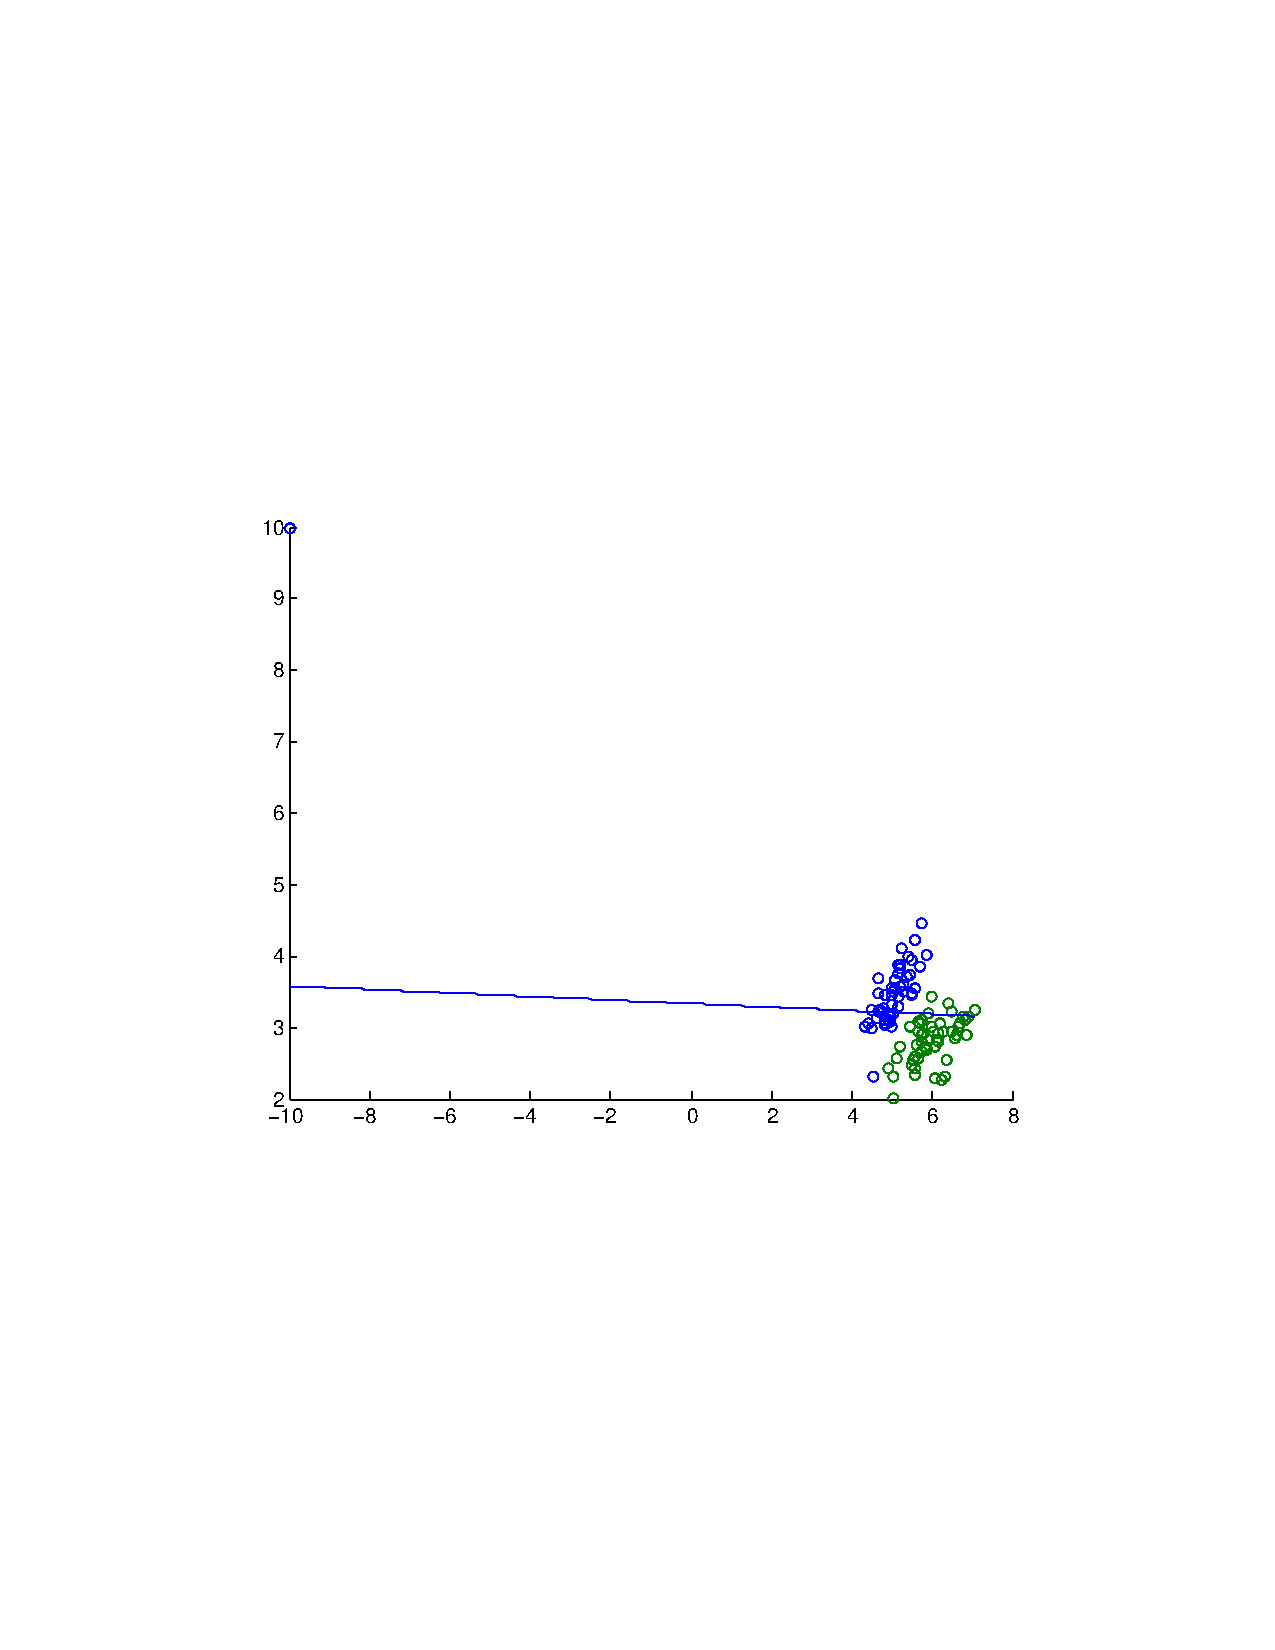
\includegraphics[width=.5\textwidth]{\figdir/prob2e_linear.pdf} \\
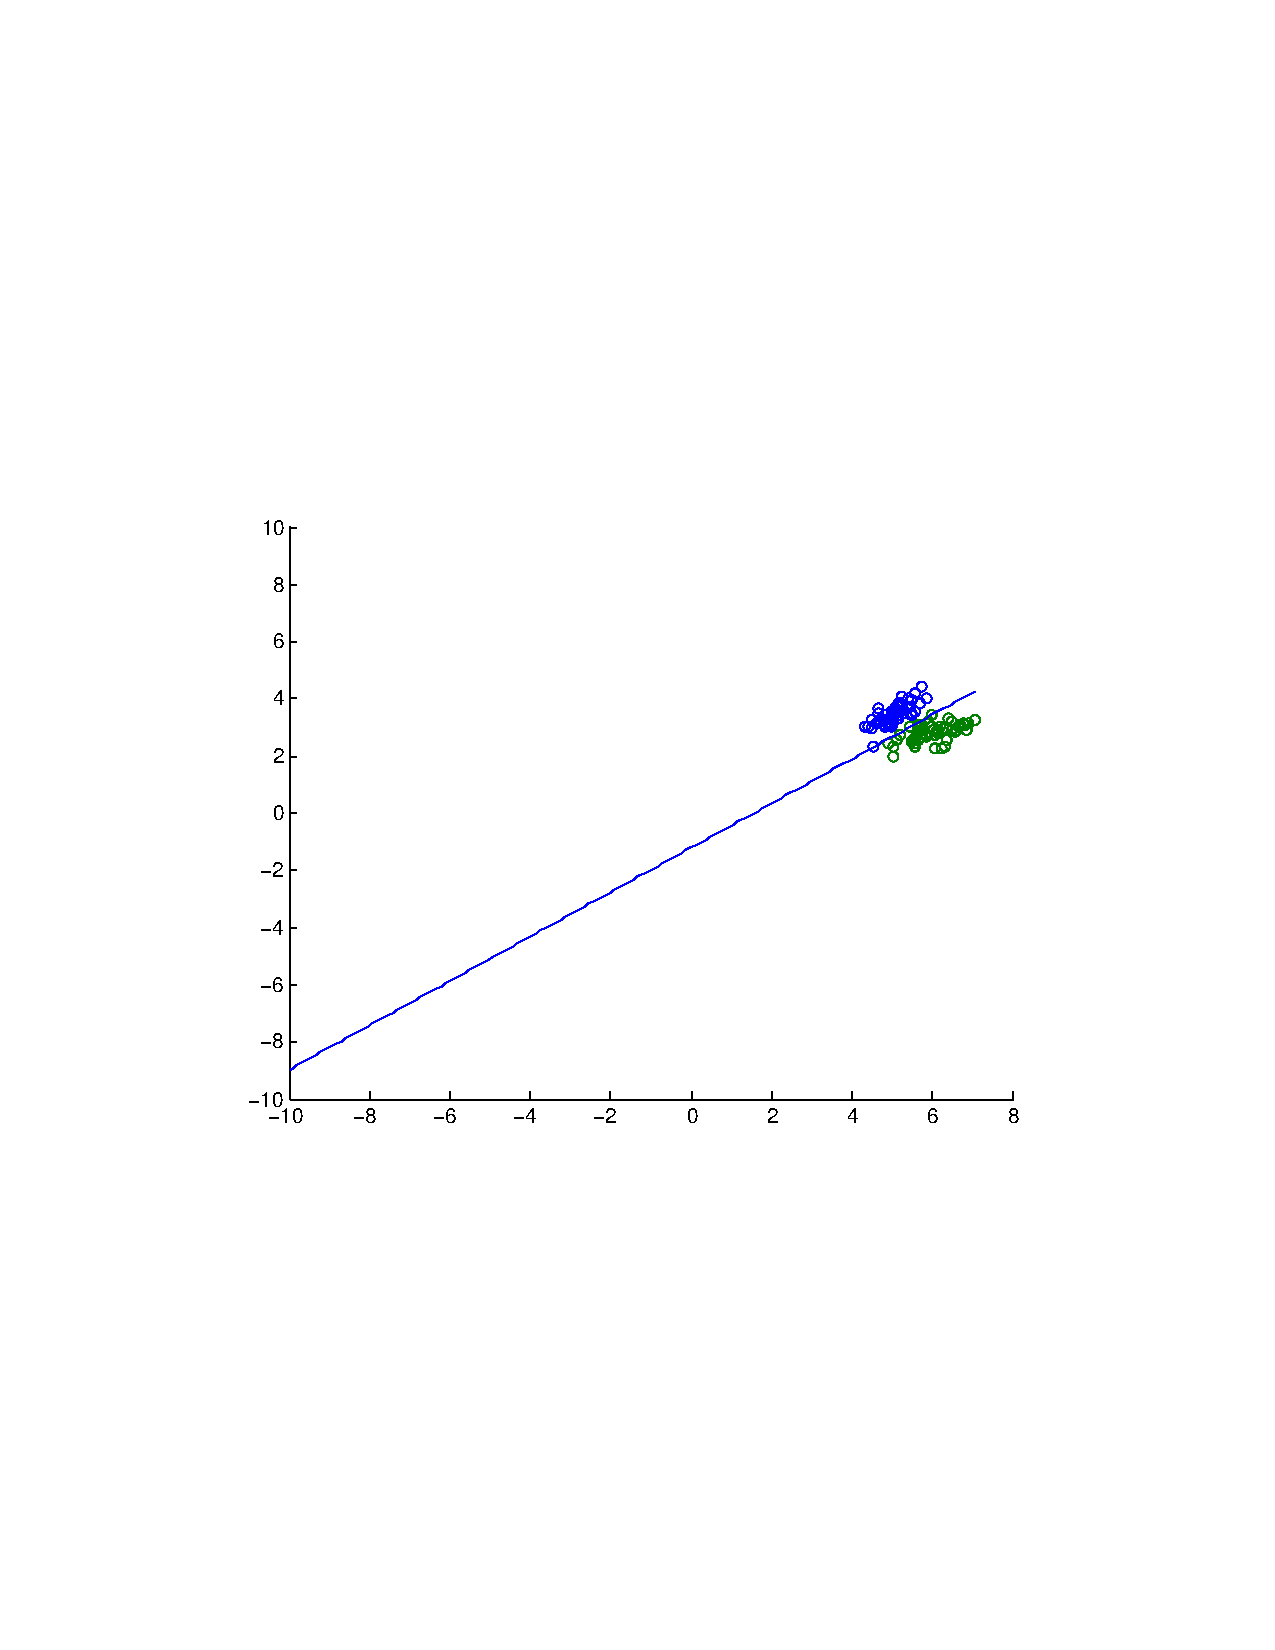
\includegraphics[width=.5\textwidth]{\figdir/prob2e_perceptron.pdf}

\end{enumerate}

% % % % % % % % % % % % % % % % % % % % % % % % % % % % % % % % % % % % % % % % % % % % % % % % % % % % % % % % % % % % % % % %

\subsection*{Problem 3: Logistic Regression}

\begin{enumerate}[(a)]
\item Done
\item See (c)

\item Using Mathematica, I derived the following:
$\frac{d J(\theta)}{d\theta} =$ $\frac{1}{m}[-y^{(j)}\log((1+\exp{-x^{(j)T}\theta'})^{-1}) - $
$(1-y^{(j)})\log(1-(1+\exp(-x^{(j)T}\theta'))^{-1}) +$ $\alpha\sum_i\theta_i^{2})]$ \\
\lstinputlisting{src/@logisticClassify/train.m}

\item 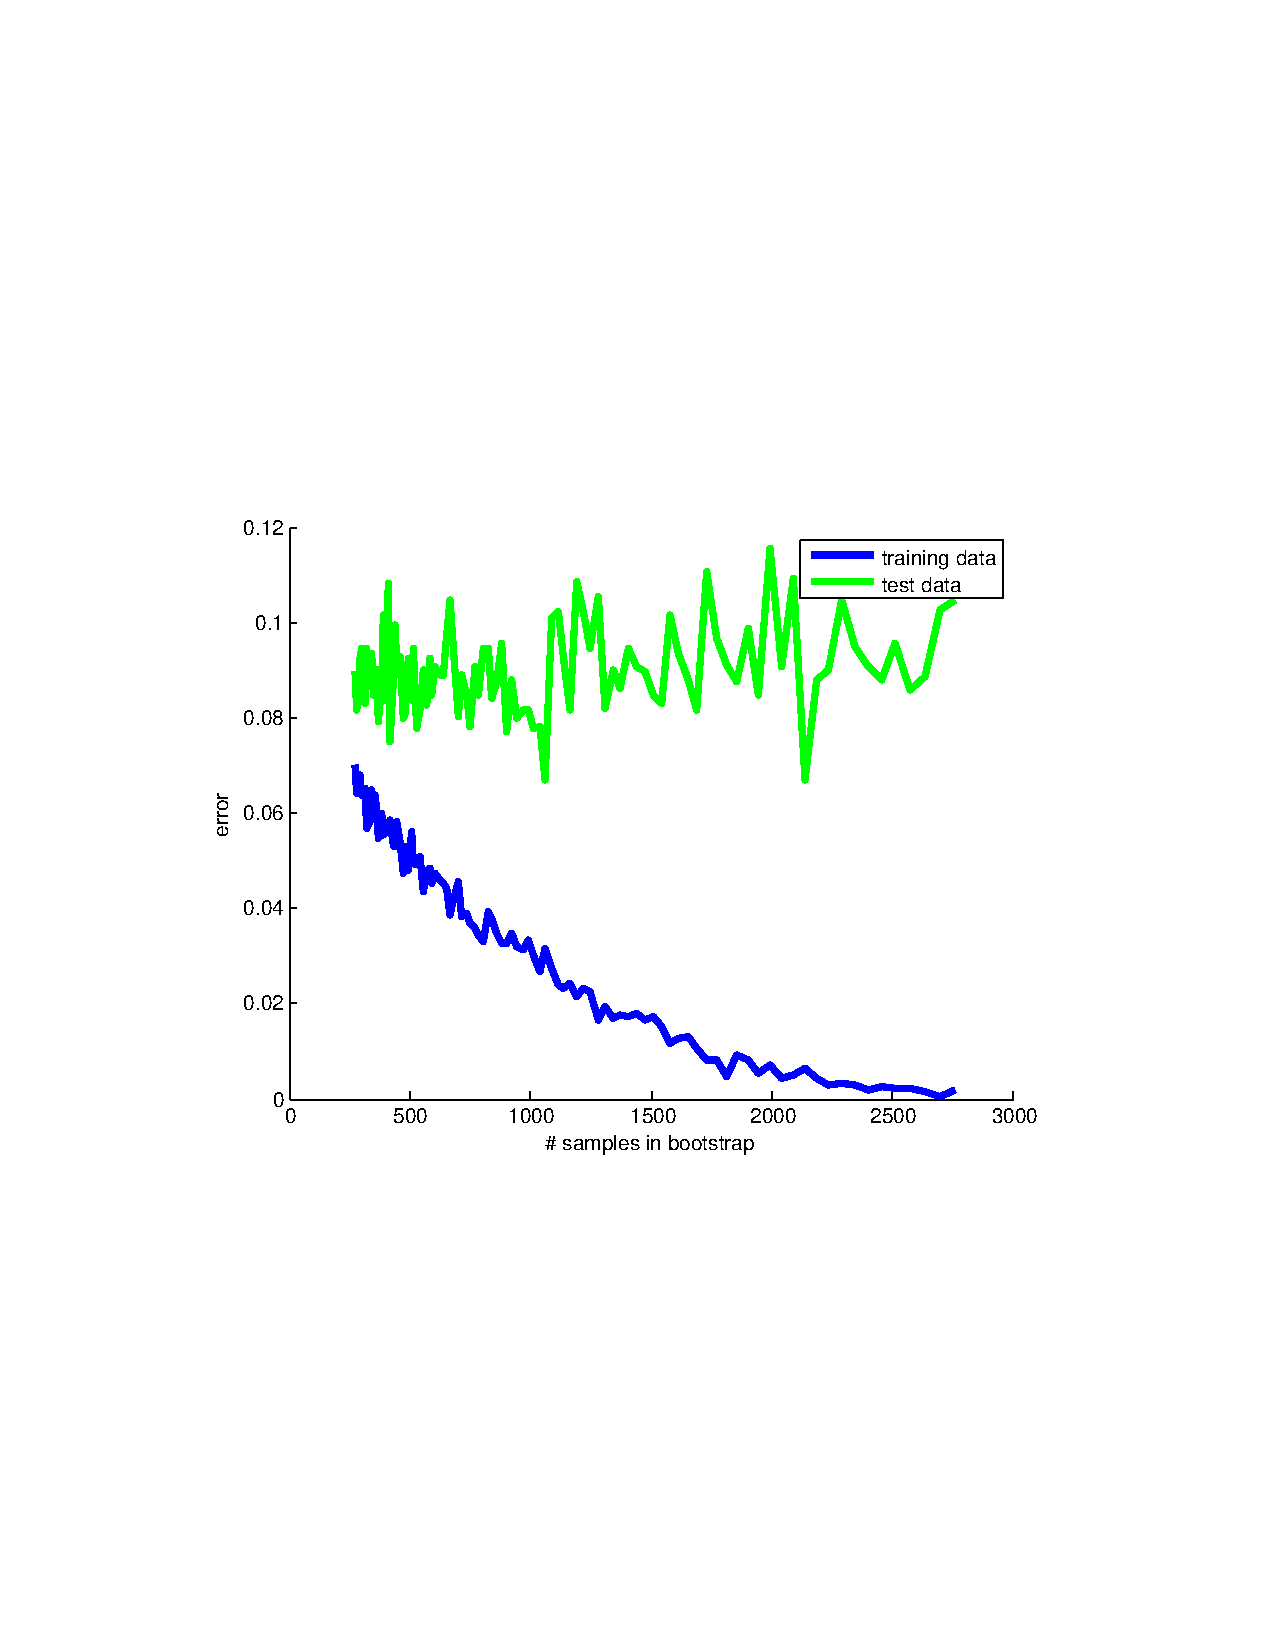
\includegraphics[width=.5\textwidth]{\figdir/prob3d.pdf}

\item On 2-d data:
\begin{figure}[h!] \centering
\begin{tabular}{cc}
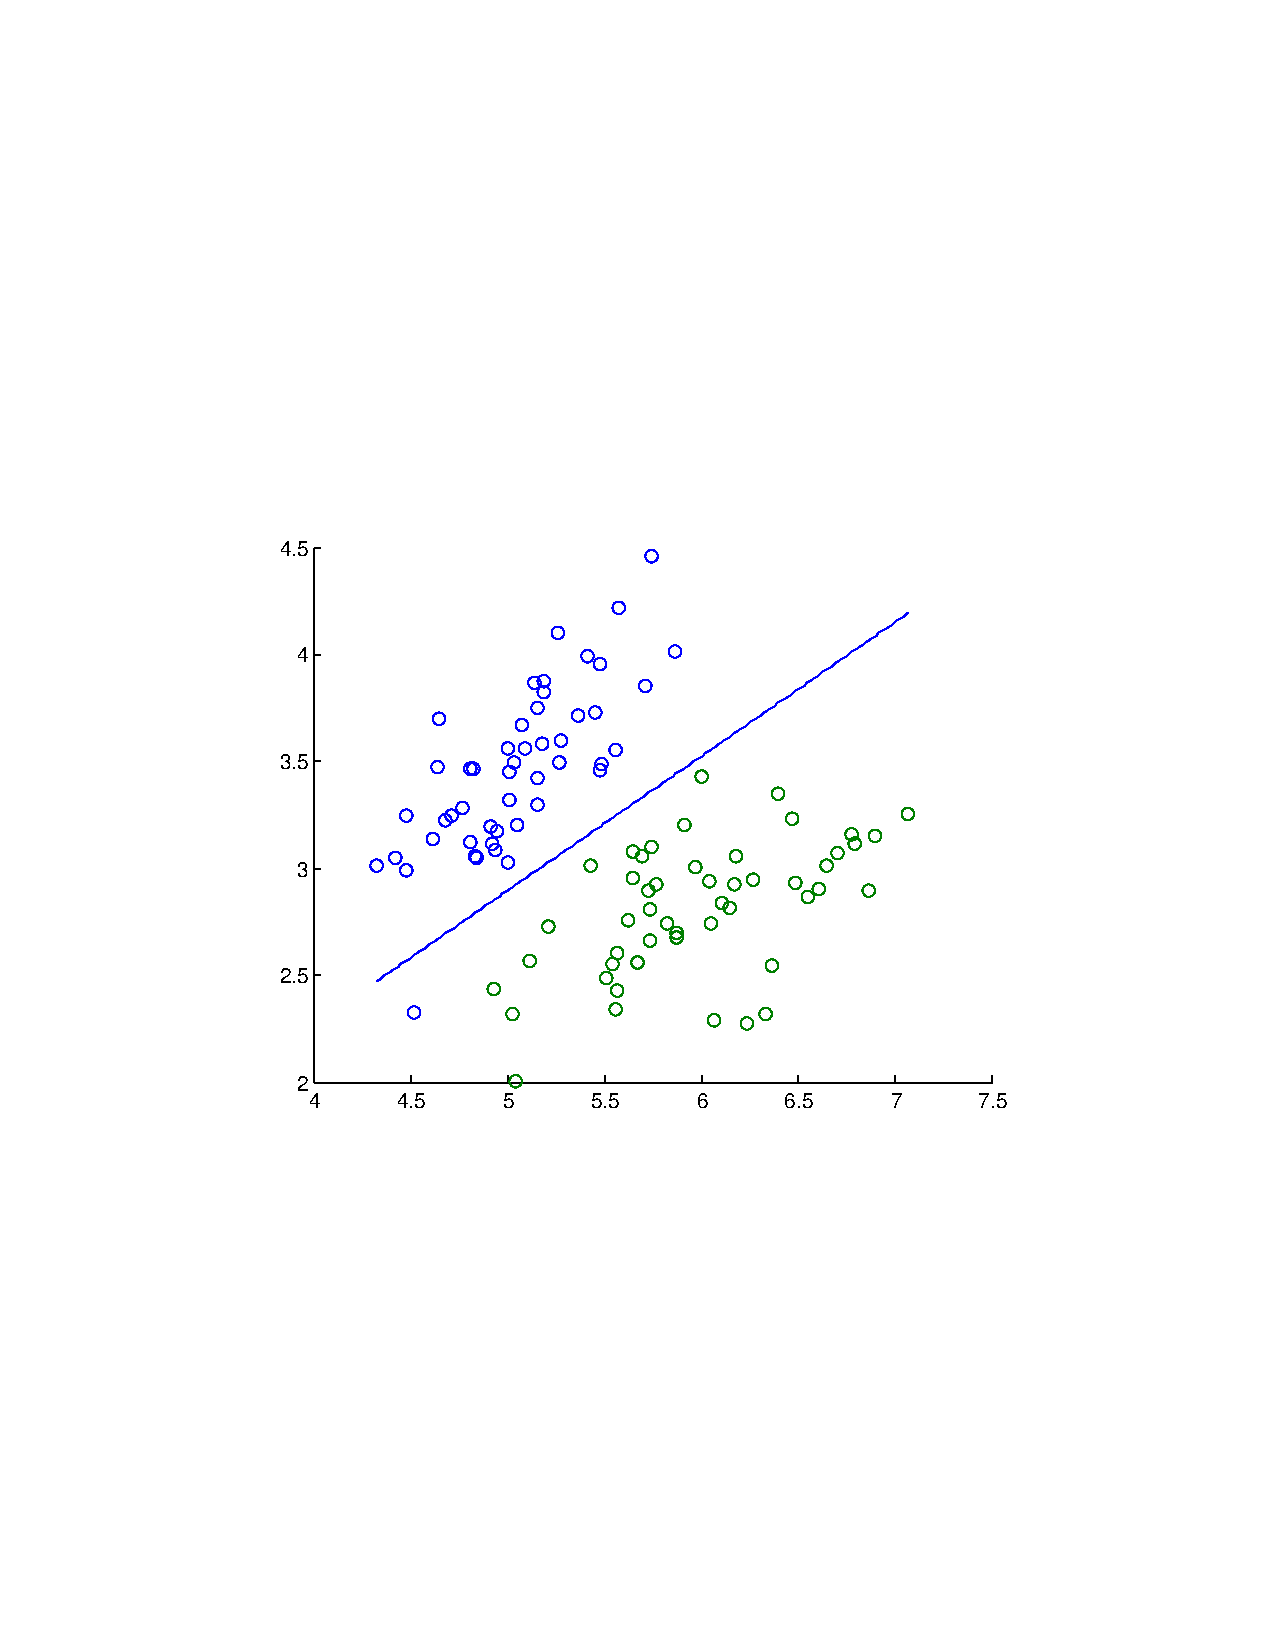
\includegraphics[width=.5\textwidth]{\figdir/prob3e_A.pdf} &
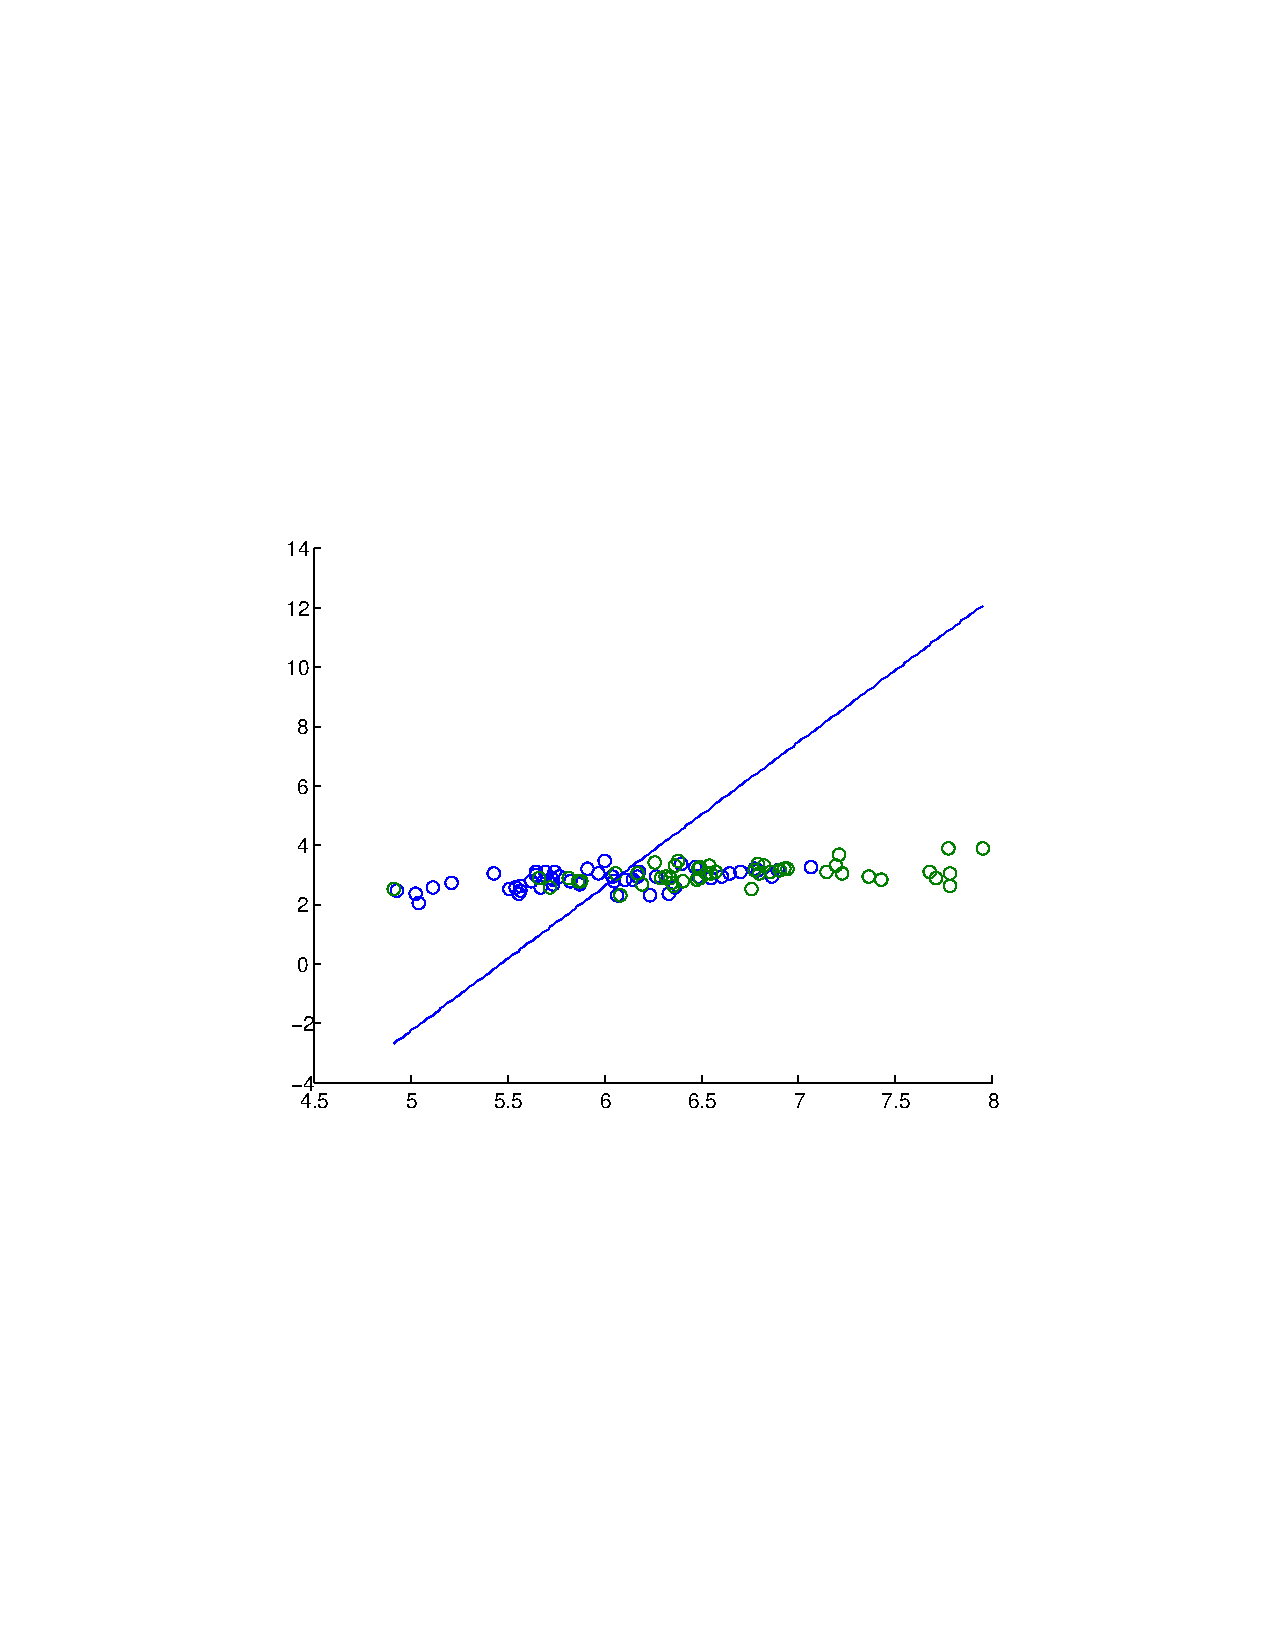
\includegraphics[width=.5\textwidth]{\figdir/prob3e_B.pdf} \\
0 vs. 1 & 1 vs. 2
\end{tabular}
\end{figure}

\item 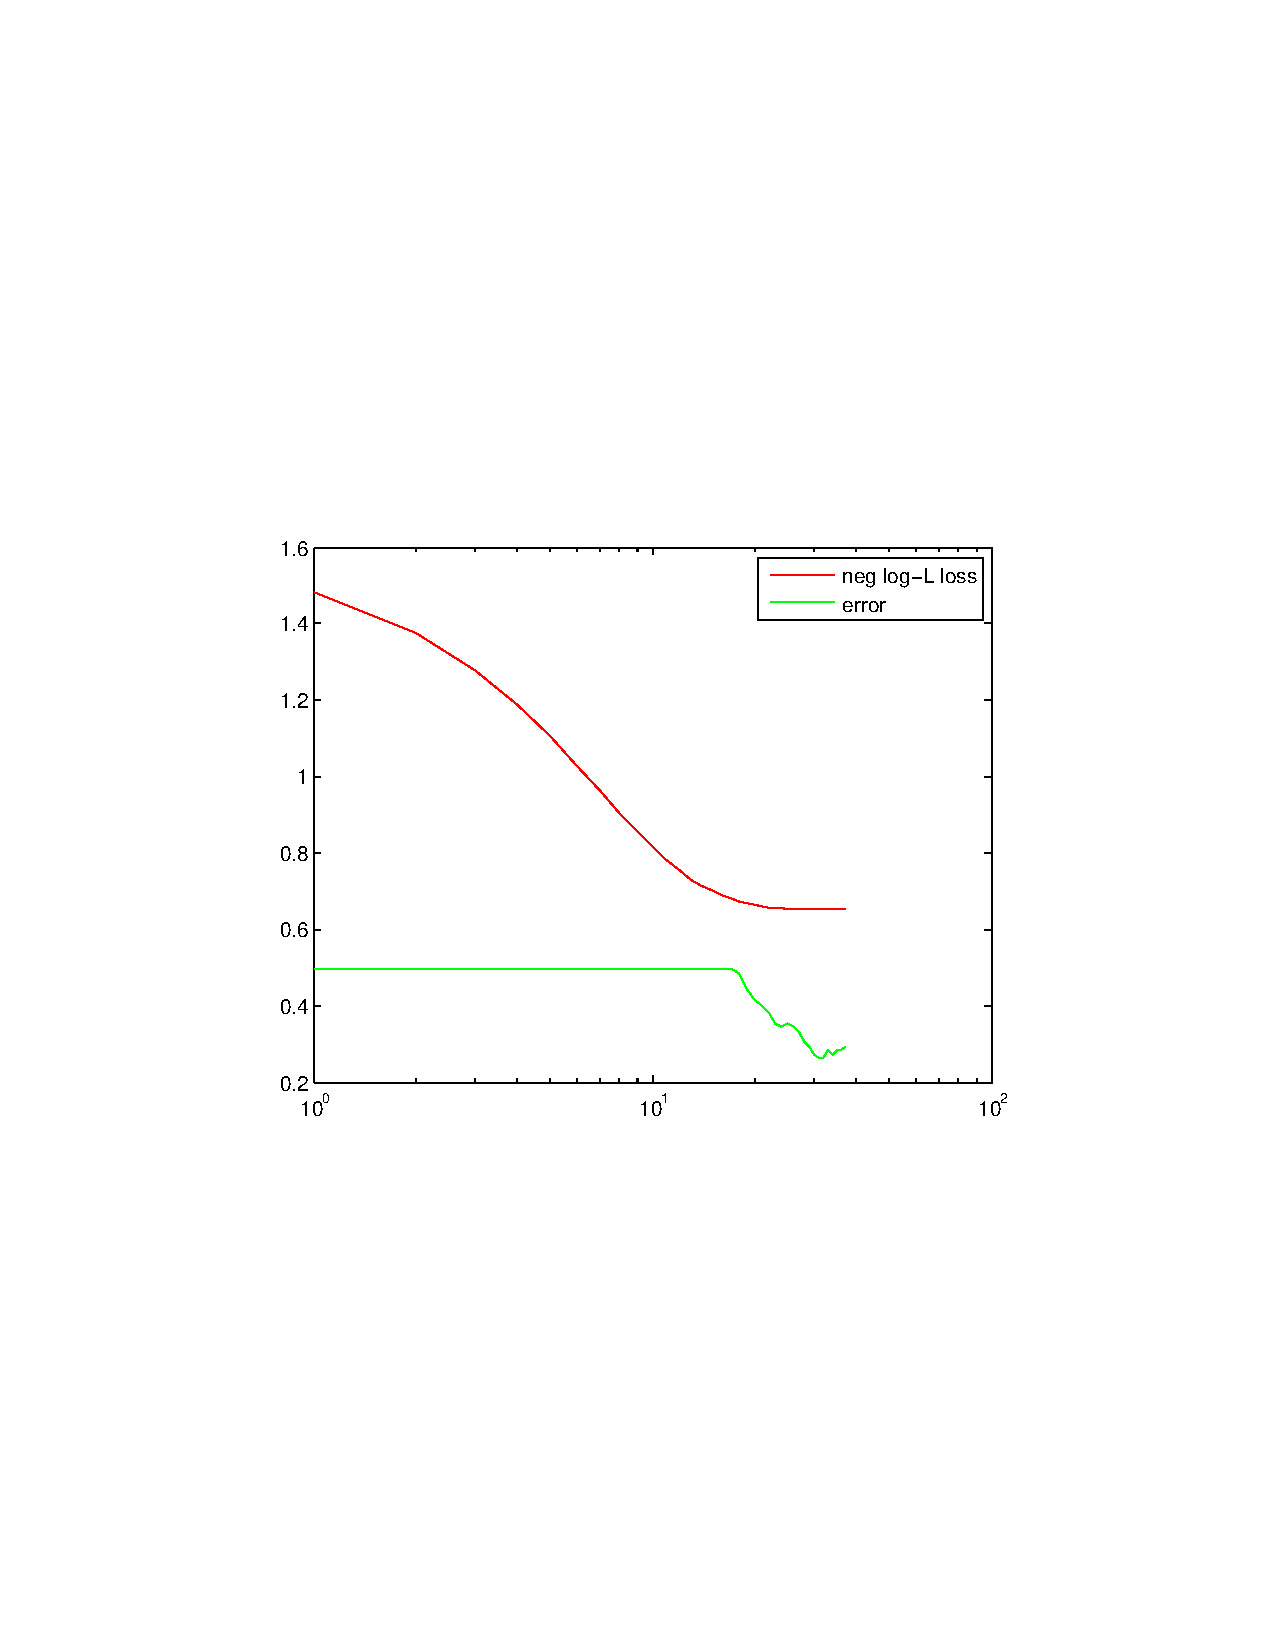
\includegraphics[width=.5\textwidth]{\figdir/prob3f_B.pdf}

\item 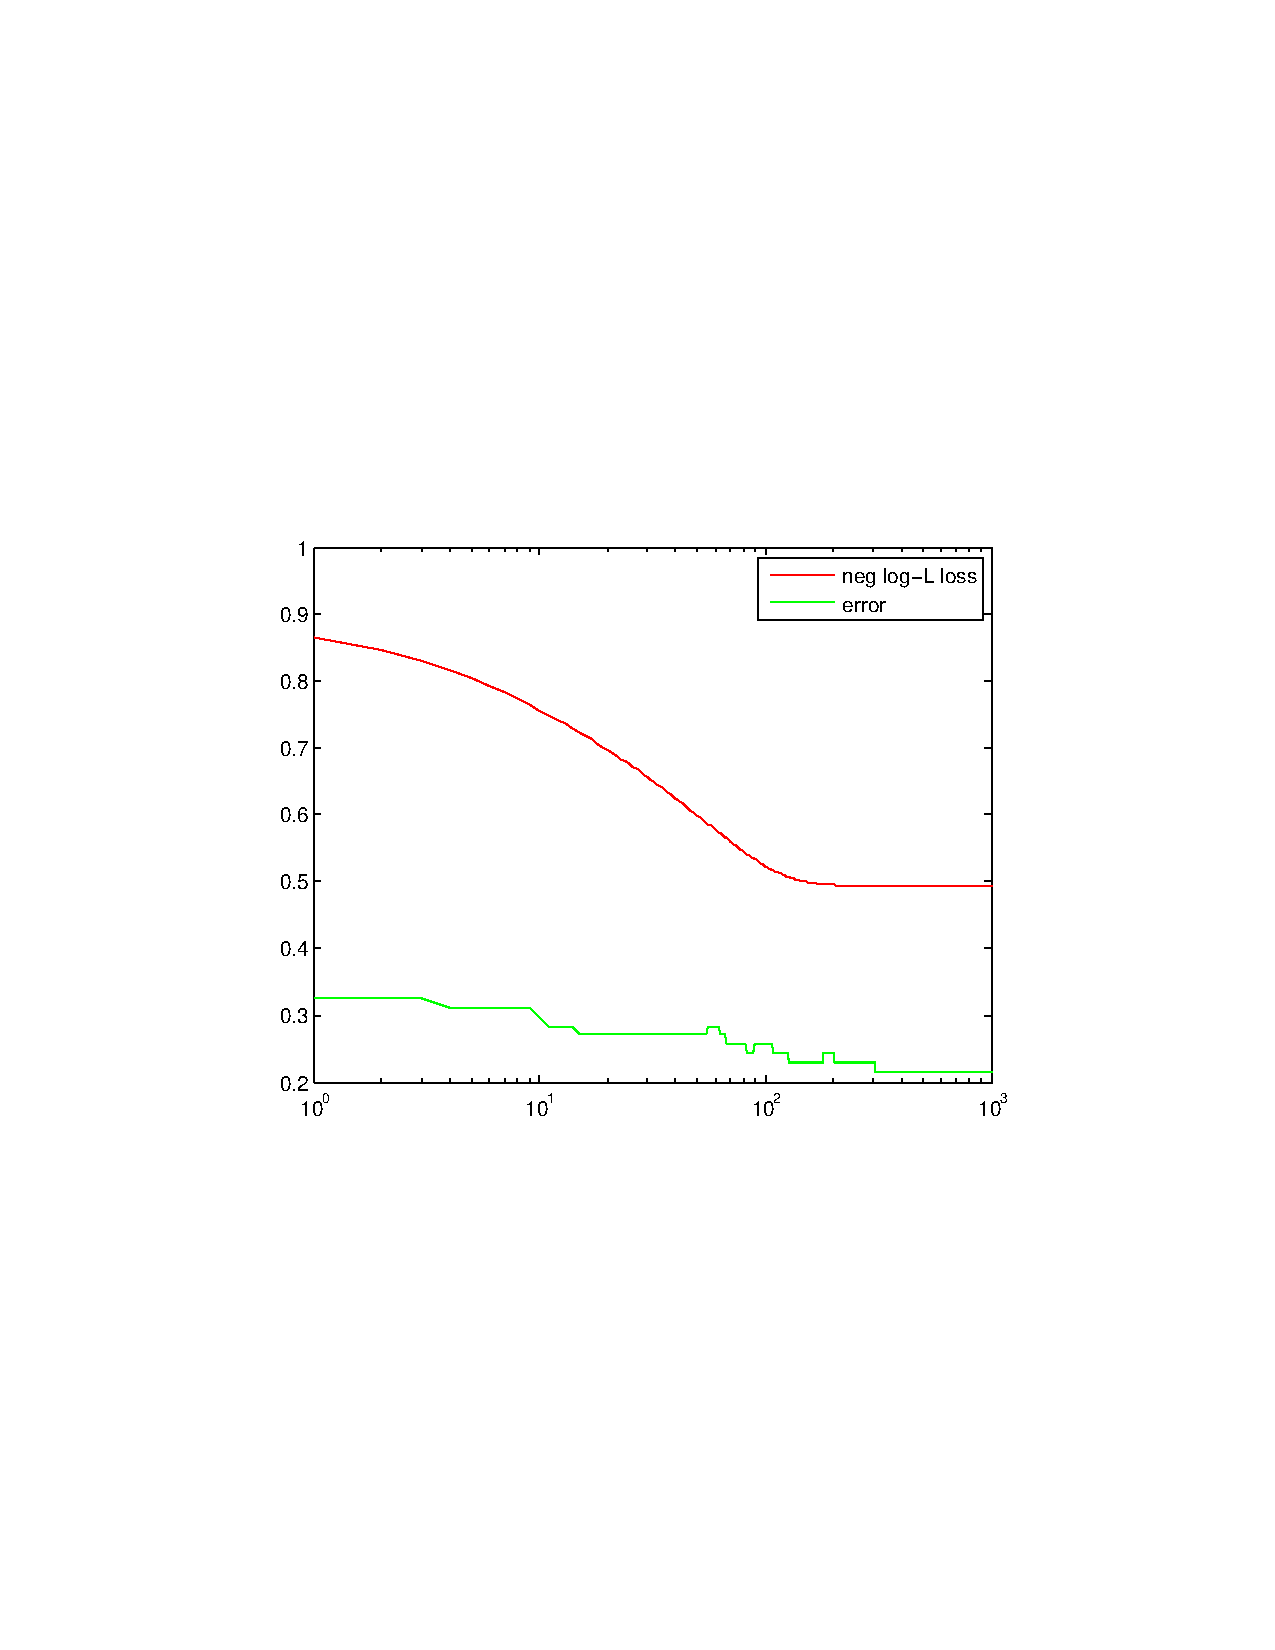
\includegraphics[width=.5\textwidth]{\figdir/prob3g.pdf} \\
training error: 0.2162 \\
test error: 0.3200

\item 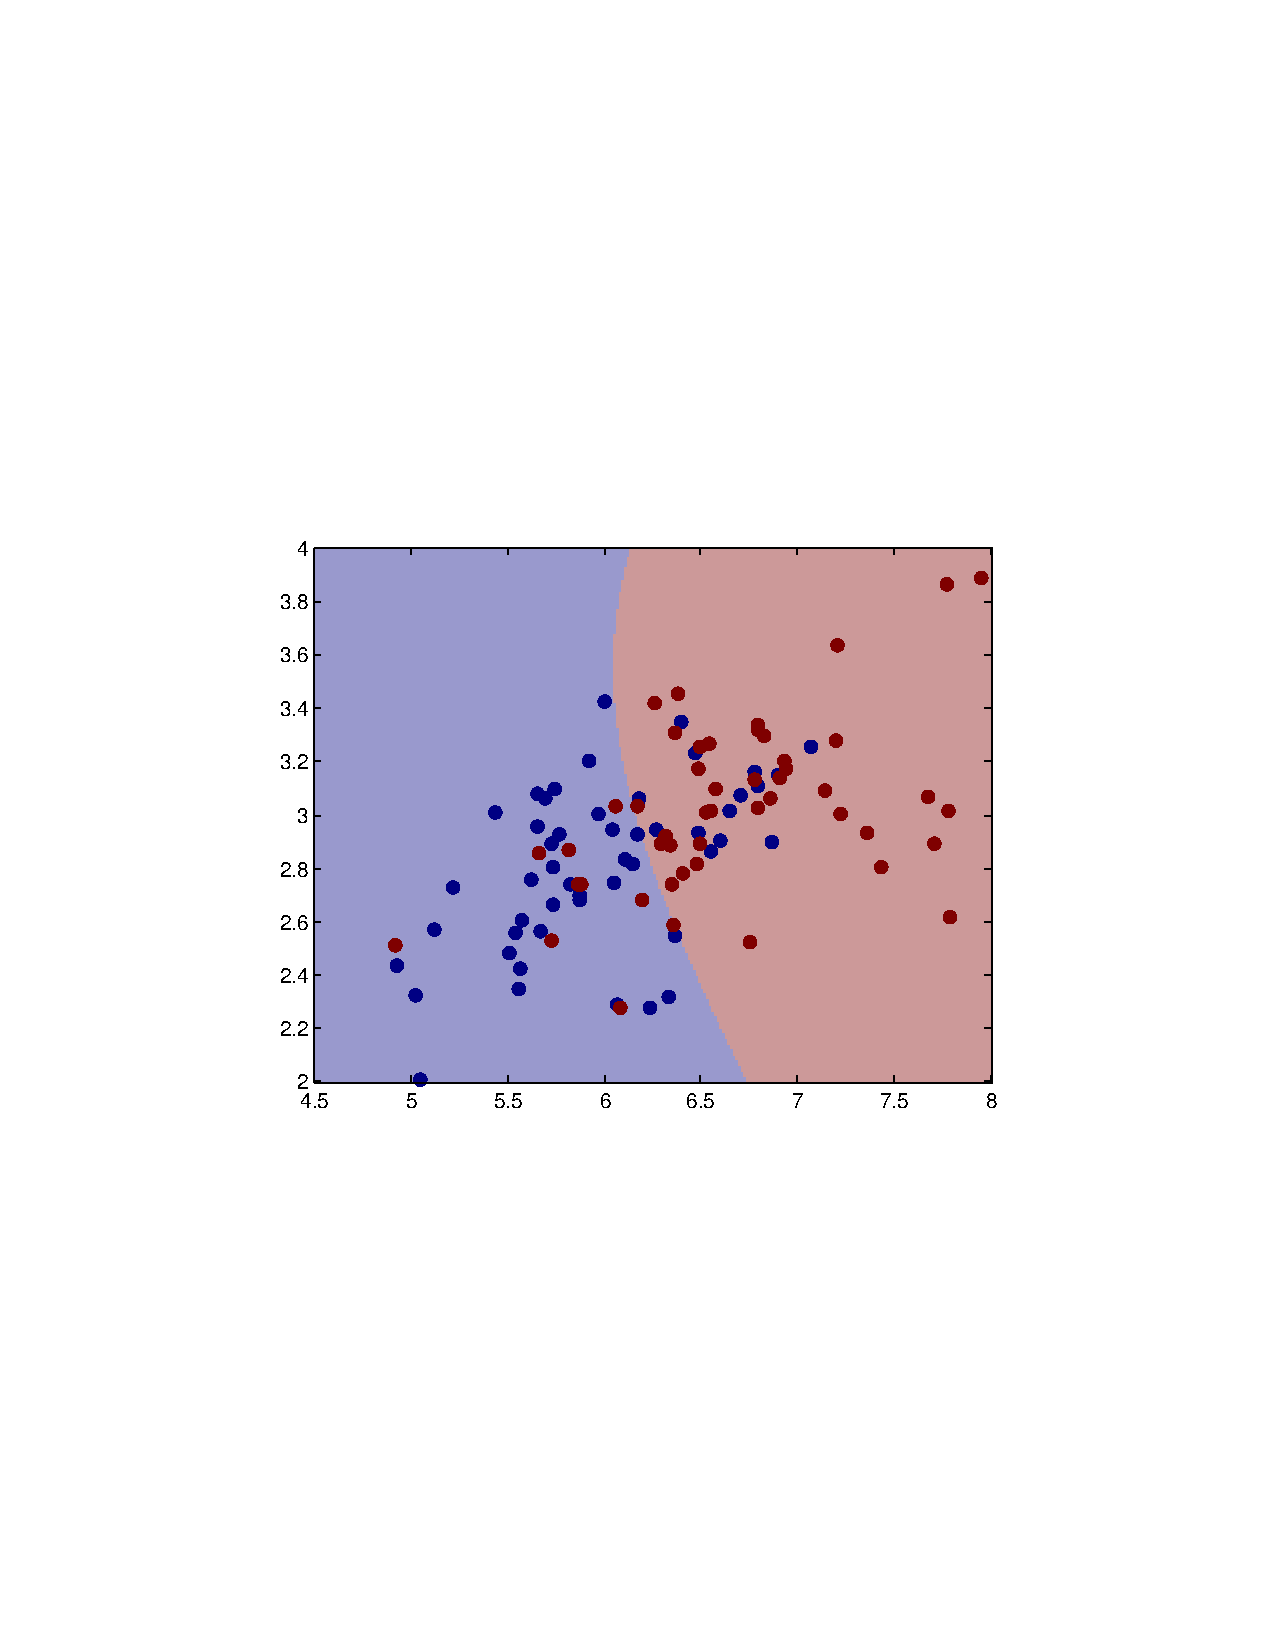
\includegraphics[width=.5\textwidth]{\figdir/prob3h.pdf}


\end{enumerate}

% % % % % % % % % % % % % % % % % % % % % % % % % % % % % % % % % % % % % % % % % % % % % % % % % % % % % % % % % % % % % % % %

\subsection*{Problem 4: High Dimensional Data}

\begin{enumerate}[(a)]
\item For settings, I used a step size of 0.1 and a maximum of 1000 iterations.
I chose these because the step size still resulted in good convergence, but would do so faster than a smaller step size.
The error rate also seemed to change very little after around 1000 iterations, almost insignificantly so.

best error: 0
best loss: 0.0016
training error: 0
test error: 0

\item Interestingly, the classifiers seem to perform quite well without all the additional features.
The error rate is slightly higher, but still seems acceptable considering how much less complex the decision algorithm will be with so many fewer features.
Furthermore, there is no difference between 2 and 10 features, so it likely takes a lot more additional features to make any significant difference in error rate.

training error 2 features: 0 \\
test error with 2 features: 0.0100 \\
training error 10 features: 0
test error 10 features: 0.0100
\end{enumerate}


\end{document}
